% !TEX program = lualatex
\documentclass[a4paper, 11pt]{article}

%% ─── Fonts ───────────────────────────────────────────────────────────────────
\usepackage{fontspec}
\usepackage{unicode-math}
\setmainfont{TeX Gyre Pagella}
\setmathfont{TeX Gyre Pagella Math}
\setsansfont[BoldFont={TeX Gyre Heros Bold}]{TeX Gyre Heros}

%% ─── Layout ──────────────────────────────────────────────────────────────────
\usepackage[a4paper, top=2.5cm, bottom=2.5cm, left=2.2cm, right=2.2cm,
            headheight=15pt]{geometry}

%% ─── Colors ──────────────────────────────────────────────────────────────────
\usepackage{xcolor}
\definecolor{DeepNavy}{HTML}{0f172a}
\definecolor{ElectricBlue}{HTML}{2563eb}
\definecolor{SkyBlueBG}{HTML}{dbeafe}
\definecolor{Amber}{HTML}{d97706}
\definecolor{AmberBG}{HTML}{fef3c7}
\definecolor{Emerald}{HTML}{059669}
\definecolor{EmeraldBG}{HTML}{d1fae5}
\definecolor{SlateGray}{HTML}{64748b}
\definecolor{LightBG}{HTML}{f8fafc}
\definecolor{CardBorder}{HTML}{e2e8f0}
\definecolor{CoralRed}{HTML}{dc2626}
\definecolor{CoralBG}{HTML}{fee2e2}
\definecolor{Purple}{HTML}{7c3aed}
\definecolor{PurpleBG}{HTML}{ede9fe}
\definecolor{Teal}{HTML}{0d9488}
\definecolor{TealBG}{HTML}{ccfbf1}

%% ─── Math ────────────────────────────────────────────────────────────────────
\usepackage{amsmath}

%% ─── Graphics & TikZ ─────────────────────────────────────────────────────────
\usepackage{graphicx}
\usepackage{tikz}
\usetikzlibrary{calc, arrows.meta, positioning, shapes.geometric}

%% ─── CircuiTikZ ──────────────────────────────────────────────────────────────
\usepackage[american]{circuitikz}
\ctikzset{resistors/scale=0.8, batteries/scale=0.8, transistors/scale=1.0}

%% ─── Tables & Lists ──────────────────────────────────────────────────────────
\usepackage{booktabs}
\usepackage{tabularx}
\usepackage{array}
\usepackage{enumitem}

%% ─── tcolorbox ───────────────────────────────────────────────────────────────
\usepackage[many, breakable]{tcolorbox}

%% ─── Headers / Titles ────────────────────────────────────────────────────────
\usepackage{fancyhdr}
\usepackage{titlesec}
\usepackage{parskip}
\usepackage{fontawesome5}
\usepackage[hidelinks]{hyperref}

%% ══════════════════════════════════════════════════════════════════════════════
%% DYNAMIC SECTION COLOUR  (set \SectionColor before each \section)
%% ══════════════════════════════════════════════════════════════════════════════
\newcommand{\SectionColor}{DeepNavy}
\newcommand{\SectionBG}{LightBG}

%% ══════════════════════════════════════════════════════════════════════════════
%% BOX STYLES
%% ══════════════════════════════════════════════════════════════════════════════

\newtcolorbox{formulabox}[1][]{enhanced, breakable,
  colback=SkyBlueBG, colframe=ElectricBlue, colbacktitle=ElectricBlue, coltitle=white,
  fonttitle=\bfseries\sffamily\small, title={\faSquareRootAlt\enspace Key Formulae},
  arc=6pt, boxrule=1.5pt, left=8pt, right=8pt, top=6pt, bottom=6pt, #1}

\newtcolorbox{solvedbox}[2][]{enhanced, breakable,
  colback=EmeraldBG, colframe=Emerald, colbacktitle=Emerald, coltitle=white,
  fonttitle=\bfseries\sffamily\small, title={\faPencilAlt\enspace Solved --- #2},
  arc=6pt, boxrule=1.5pt, left=8pt, right=8pt, top=6pt, bottom=6pt, #1}

\newtcolorbox{conceptbox}[1][Key Concept]{enhanced,
  colback=PurpleBG, colframe=Purple, colbacktitle=Purple, coltitle=white,
  fonttitle=\bfseries\sffamily\small, title={\faLightbulb\enspace #1},
  arc=6pt, boxrule=1.5pt, left=8pt, right=8pt, top=6pt, bottom=6pt}

\newtcolorbox{warnbox}{enhanced,
  colback=CoralBG, colframe=CoralRed, colbacktitle=CoralRed, coltitle=white,
  fonttitle=\bfseries\sffamily\small,
  title={\faExclamationTriangle\enspace Exam Traps --- Don't Lose Marks Here},
  arc=6pt, boxrule=1.5pt, left=8pt, right=8pt, top=6pt, bottom=6pt}

\newtcolorbox{stepsbox}[1][Analysis Steps]{enhanced,
  colback=TealBG, colframe=Teal, colbacktitle=Teal, coltitle=white,
  fonttitle=\bfseries\sffamily\small, title={\faListOl\enspace #1},
  arc=6pt, boxrule=1.5pt, left=8pt, right=8pt, top=6pt, bottom=6pt}

%% Circuit tint box — coloured background behind each circuit diagram
%% Usage: \begin{circbox}[BG-colour]{Frame-colour} ... \end{circbox}
\newtcolorbox{circbox}[2][LightBG]{
  enhanced, colback=#1, colframe=#2,
  arc=6pt, boxrule=0.8pt, left=5pt, right=5pt, top=5pt, bottom=5pt}

%% ══════════════════════════════════════════════════════════════════════════════
%% SECTION STYLING  (reads \SectionColor set before each \section call)
%% ══════════════════════════════════════════════════════════════════════════════

\newcommand{\secunderline}{%
  \color{\SectionColor}\vspace{2pt}\titlerule[1.5pt]\vspace{4pt}}

\titleformat{\section}
  {\Large\bfseries\sffamily\color{\SectionColor}}{\thesection}{1em}{}[\secunderline]
\titleformat{\subsection}
  {\large\bfseries\sffamily\color{\SectionColor}}{\thesubsection}{1em}{}
\titleformat{\subsubsection}
  {\normalsize\bfseries\sffamily\color{SlateGray}}{}{0em}{}
\titlespacing{\section}{0pt}{20pt}{8pt}
\titlespacing{\subsection}{0pt}{12pt}{4pt}

%% ══════════════════════════════════════════════════════════════════════════════
%% HEADER
%% ══════════════════════════════════════════════════════════════════════════════
\pagestyle{fancy}
\fancyhf{}
\renewcommand{\headrulewidth}{0pt}
\fancyhead[L]{%
  
\begin{tikzpicture}[remember picture, overlay]
    \fill[DeepNavy] (0,0) rectangle (\paperwidth, 0.55cm);
    \node[anchor=west, text=white, font=\small\sffamily, inner sep=6pt]
      at (0,0.28cm) {EEE F111 --- Electrical Sciences \textbf{Master Pack}};
    \node[anchor=east, text=SlateGray!60!white, font=\small\sffamily, inner sep=6pt]
      at (\paperwidth-2.2cm,0.28cm) {\thepage};
  \end{tikzpicture}}

%% ══════════════════════════════════════════════════════════════════════════════
%% HELPERS
%% ══════════════════════════════════════════════════════════════════════════════

%% Styled badge: red pill showing exam frequency
\newcommand{\examfreq}[1]{\hfill
  \tikz[baseline=-0.6ex]\node[fill=CoralRed, text=white,
    font=\bfseries\sffamily\scriptsize, inner sep=3.5pt,
    rounded corners=4pt]{\faFire\ \ #1\,/\,6 exams};}
%% Silence \examfreq in PDF bookmarks; sections use \section[short]{long\examfreq{}} to protect TOC
\pdfstringdefDisableCommands{\def\examfreq#1{}}

\newcommand{\ans}[1]{\boxed{#1}}
\newcommand{\step}[1]{\par\smallskip\textcolor{Teal}{\textbf{Step #1.}}\enspace}

%% ══════════════════════════════════════════════════════════════════════════════
%% DOCUMENT
%% ══════════════════════════════════════════════════════════════════════════════
\begin{document}

%% ─── TITLE PAGE ──────────────────────────────────────────────────────────────
\thispagestyle{empty}

\begin{tikzpicture}[remember picture, overlay]
  \fill[DeepNavy]
    (current page.north west) rectangle ($(current page.north east)+(0,-10cm)$);
  %% Subtle circuit-trace decoration
  \begin{scope}[opacity=0.07, DeepNavy!40!ElectricBlue, line width=0.6pt]
    \draw (1,-1) -- (1,-4) -- (4,-4) -- (4,-7);
    \draw (4,-4) -- (8,-4) -- (8,-6);
    \draw (3,-2) -- (6,-2) -- (6,-5) -- (9,-5);
    \draw (2,-6) -- (5,-6) -- (5,-9);
    \draw (7,-3) -- (10,-3) -- (10,-8) -- (13,-8);
    \draw (12,-2) -- (12,-5) -- (15,-5);
    \draw (14,-1) -- (14,-3) -- (17,-3) -- (17,-7);
    \draw (16,-4) -- (19,-4);
    \foreach \x/\y in {1/-1, 4/-4, 8/-6, 3/-2, 6/-5, 2/-6, 10/-8, 12/-5, 14/-3, 17/-7}
      \filldraw (\x,\y) circle(1.8pt);
  \end{scope}
  \fill[ElectricBlue]
    ($(current page.north west)+(0,-10cm)$) rectangle
    ($(current page.north east)+(0,-10.28cm)$);
  \fill[Amber]
    ($(current page.north west)+(0,-10.28cm)$) rectangle
    ($(current page.north east)+(0,-10.50cm)$);
  \fill[LightBG]
    (current page.south west) rectangle ($(current page.south east)+(0,2.2cm)$);
  \node[anchor=south, text=SlateGray, font=\footnotesize\sffamily]
    at ($(current page.south)+(0,0.8cm)$)
    {BITS Pilani \textbullet\ EEE F111 \textbullet\ Electrical Sciences \textbullet\ 2023--2025};
\end{tikzpicture}

\vspace*{2.8cm}
\begin{center}
  {\large\sffamily\color{ElectricBlue!70!white}%
    {\addfontfeatures{LetterSpace=15}BITS PILANI}}\\[0.5cm]
  {\small\sffamily\color{white!60!DeepNavy} EEE F111 --- Electrical Sciences}\\[1.5cm]
  {\fontsize{38}{46}\selectfont\bfseries\sffamily\color{white}
    Comprehensive Exam\\[0.3cm] Master Pack}\\[1cm]
  {\large\sffamily\color{white!80!DeepNavy}
    Formula Reference \textbullet\ Circuit Diagrams \textbullet\ Solved Past Papers\\[0.3cm]
    \textit{All 6 Comprehensive Exams (2023--2025)}}
\end{center}

\vspace{3.5cm}
\begin{center}
\begin{tcolorbox}[enhanced, width=0.82\textwidth, colback=white,
  colframe=CardBorder, arc=8pt, boxrule=1pt,
  left=14pt, right=14pt, top=10pt, bottom=10pt]
  \centering\small\sffamily\color{SlateGray}
  \textbf{\faFire\ Topics by Exam Frequency}\\[8pt]
  \begin{tabular}{@{}lccc@{}}
    \toprule
    \textbf{Topic} & \textbf{Freq} & \textbf{Hours} & \textbf{Status}\\
    \midrule
    Bipolar Junction Transistors (BJTs) & 6/6 & 3h & \textcolor{Emerald}{\faCheckCircle} \\
    Diodes (PN Junction + Zener)        & 6/6 & 5h & \textcolor{Emerald}{\faCheckCircle} \\
    AC Circuits + 3-Phase               & 6/6 & 7h & \textcolor{Emerald}{\faCheckCircle} \\
    DC Circuits + Network Theorems      & 5/6 & 5h & \textcolor{Emerald}{\faCheckCircle} \\
    MOSFETs / JFETs                     & 5/6 & 3h & \textcolor{Emerald}{\faCheckCircle} \\
    Transformers + Magnetic Circuits    & 5/6 & 5h & \textcolor{Amber}{\faClock} \\
    Op-Amps                             & 4/6 & 2h & \textcolor{Amber}{\faClock} \\
    Filters + Resonance                 & 4/6 & 2h & \textcolor{Amber}{\faClock} \\
    \bottomrule
  \end{tabular}
\end{tcolorbox}
\end{center}

\newpage\tableofcontents\newpage

%% ══════════════════════════════════════════════════════════════════════════════
%% ── SECTION 1: BJTs  (Blue)
\renewcommand{\SectionColor}{ElectricBlue}
\renewcommand{\SectionBG}{SkyBlueBG}
\section[Bipolar Junction Transistors (BJTs)]{Bipolar Junction Transistors (BJTs)\examfreq{6}}
%% ══════════════════════════════════════════════════════════════════════════════

\subsection{Operating Regions}

\begin{center}\renewcommand{\arraystretch}{1.3}
\begin{tabular}{lllll}
\toprule
\textbf{Region} & \textbf{E-B Jn.} & \textbf{C-B Jn.} & \textbf{Role} & \textbf{Check} \\
\midrule
Active     & Forward & Reverse & Amplifier    & $V_{CE}>0.2\ \text{V}$  \\
Saturation & Forward & Forward & Switch (ON)  & $h_{FE}I_B\geq I_C$ \\
Cutoff     & Reverse & Reverse & Switch (OFF) & $V_{BE}<0.5\ \text{V}$ \\
\bottomrule
\end{tabular}
\end{center}

\begin{conceptbox}[Si BJT Approximations]
Active: $V_{BE}=0.7\ \text{V}$ \enspace\textbullet\enspace
Saturation: $V_{BE}=0.8\ \text{V}$,\ $V_{CE}=0.2\ \text{V}$ \enspace\textbullet\enspace
Cutoff: all currents $=0$
\end{conceptbox}

\subsection{Key Formulae}

\begin{formulabox}
\begin{align*}
  I_E &= I_B + I_C \\
  I_C &= \beta I_B \quad\text{(active mode)} \\
  \beta &= \frac{\alpha}{1-\alpha},\qquad \alpha=\frac{\beta}{\beta+1} \\
  I_B &= \frac{V_{BB}-V_{BE}}{R_B+(1+\beta)R_E} \\
  V_{CE} &= V_{CC} - I_C R_C - I_E R_E
\end{align*}
\textbf{Saturation check:} $h_{FE}I_B\geq I_{C(\text{sat})}$
where $I_{C(\text{sat})}=\dfrac{V_{CC}-V_{CE(\text{sat})}}{R_C}$
\end{formulabox}

\begin{stepsbox}[Standard DC Analysis]
\begin{enumerate}[noitemsep,topsep=0pt]
  \item Assume active; set $V_{BE}=0.7\ \text{V}$; KVL base loop $\to$ $I_B$
  \item $I_C=\beta I_B$,\quad $I_E=I_B+I_C$
  \item KVL collector loop $\to$ $V_{CE}$
  \item Verify $V_{CE}>0.2\ \text{V}$; if not, redo assuming saturation.
\end{enumerate}
\end{stepsbox}

\subsection{Solved Past Exam Questions}

%% ── 2023 ──────────────────────────────────────────────────────────────────────
\begin{solvedbox}{Comp.\ Exam 2023 --- Two-NPN Cascade}
\noindent\begin{minipage}[t]{0.40\linewidth}
\vspace{0pt}
\begin{circbox}[SkyBlueBG]{ElectricBlue!30}
\centering
\begin{circuitikz}[american, scale=0.72, transform shape]
  \draw (0,0) node[npn](Q1){\small$Q_1$};
  \draw (3.6,0) node[npn](Q2){\small$Q_2$};
  \draw (Q1.base)
    to[R, l=$R_B$] (-2.2,0)
    to[battery1, invert, l_=$V_{BB}$] (-2.2,-2.5) node[ground]{};
  \draw (Q1.collector)
    to[R, l=$R_{C1}$] (0,2.5) node[vcc]{$V_{CC}$};
  \draw (Q1.collector) to[short,*-] (0,1.1) -| (Q2.base);
  \draw (Q2.collector) to[short] (3.6,2.5) node[vcc]{$V_{CC}$};
  \draw (Q1.emitter) to[short] (0,-1.0) to[short] (1.6,-1.0)
    to[R, l_=$R_E$] (1.6,-3.0) node[ground]{};
  \draw (Q2.emitter) to[short] (3.6,-1.0) to[short] (1.6,-1.0);
\end{circuitikz}

\vspace{4pt}
{\footnotesize $\beta=100$,\ $R_B=230\text{k}$,\ $R_{C1}=1\text{k}$,\\
$R_E=2\text{k}$,\ $V_{BB}=3\text{V}$,\ $V_{CC}=6\text{V}$}
\end{circbox}
\end{minipage}%
\hfill%
\begin{minipage}[t]{0.56\linewidth}
\vspace{0pt}
\textbf{(i)} Assume both active; $\beta=100$, $V_{BE}=0.7\ \text{V}$

\step{1}
\[
I_{B1}=\frac{V_{BB}-V_{BE}}{R_B+(1+\beta)R_E}=\frac{2.3}{432\text{k}}=5.32\ \mu\text{A}
\]
\step{2}
$\ans{i_{C1}=\beta I_{B1}=0.532\ \text{mA}}$

\step{3} $I_{E1}=101\times5.32=537\ \mu\text{A}$
\[
\ans{v_{CE1}=6-0.532(1)-0.537(2)=4.39\ \text{V}}\ \checkmark
\]
\step{4} $V_{B2}=V_{C1}=5.468\ \text{V}$;
$\ans{v_{E2}=5.468-0.7=4.768\ \text{V}}$

\textbf{(ii)} At $V_{BB}=13\ \text{V}$ ($Q_1$ saturates):
\[
I_{C(\text{sat})}=\frac{5.8}{1\text{k}}=5.8\ \text{mA}\quad
\ans{h_{FE(\min)}\approx110}
\]
\end{minipage}
\end{solvedbox}

%% ── 2024 Feb ─────────────────────────────────────────────────────────────────
\begin{solvedbox}{Comp.\ Exam 2024 (Feb) --- Two-Stage CE Amplifier}
\noindent\begin{minipage}[t]{0.40\linewidth}
\vspace{0pt}
\begin{circbox}[SkyBlueBG]{ElectricBlue!30}
\centering
\begin{circuitikz}[american, scale=0.72, transform shape]
  \draw (0,0) node[npn](T1){\small$T_1$};
  \draw (3.6,0) node[npn](T2){\small$T_2$};
  \draw (T1.base) to[R, l=$150\text{k}$] (-2,0) node[vcc]{$12\text{V}$};
  \draw (T1.collector) to[R, l=$1\text{k}$] (0,2.5) node[vcc]{$V_{CC}$};
  \draw (T1.collector) to[short,*-] (0,1.0) -| (T2.base);
  \draw (T2.collector) to[R, l=$1\text{k}$] (3.6,2.5) node[vcc]{$V_{CC}$};
  \draw (T1.emitter) to[R, l_=$330\Omega$] (0,-2.5) node[ground]{};
  \draw (T2.emitter) to[R, l_=$1\text{k}$] (3.6,-2.5) node[ground]{};
\end{circuitikz}
\end{circbox}
\end{minipage}%
\hfill%
\begin{minipage}[t]{0.56\linewidth}
\vspace{0pt}
$\beta=120$, $V_{CC}=12\ \text{V}$.

\step{1}
\[
I_{B1}=\frac{12-0.7}{150\text{k}+(121)(0.33\text{k})}=59.5\ \mu\text{A}
\]
\step{2} $I_{C1}=7.14\ \text{mA}$, $I_{E1}=7.2\ \text{mA}$
\[
\ans{V_{CE1}=12-7.14(1)-7.2(0.33)=2.48\ \text{V}}
\]
\step{3} $V_{B2}=12-7.14=4.86\ \text{V}$;
$I_{B2}=34.1\ \mu\text{A}$, $I_{C2}=4.09\ \text{mA}$
\[
\ans{V_{CE2}=12-4.09(1)-4.12(1)=3.79\ \text{V}}
\]
\end{minipage}
\end{solvedbox}

%% ── 2024 May ─────────────────────────────────────────────────────────────────
\begin{solvedbox}{Comp.\ Exam 2024 (May) --- Min $h_{FE}$ for Saturation}
\noindent\begin{minipage}[t]{0.40\linewidth}
\vspace{0pt}
\begin{circbox}[SkyBlueBG]{ElectricBlue!30}
\centering
\begin{circuitikz}[american, scale=0.72, transform shape]
  \draw (0,0) node[npn](Q1){\small$Q_1$};
  \draw (3.6,0) node[npn](Q2){\small$Q_2$};
  \draw (Q1.base) to[R, l=$68\text{k}$] (-2.2,0) node[vcc]{$5\text{V}$};
  \draw (Q1.collector) to[R, l=$1\text{k}$] (0,2.5) node[vcc]{$5\text{V}$};
  \draw (Q1.collector) to[short,*-] (0,1.1) -| (Q2.base);
  \draw (Q2.collector) to[R, l=$500\Omega$] (3.6,2.5) node[vcc]{$5\text{V}$};
  \draw (Q1.emitter) to[R, l_=$210\Omega$] (0,-2.5) node[ground]{};
  \draw (Q2.emitter) to[short] (3.6,-1.2) to[short] (0,-1.2);
\end{circuitikz}
\end{circbox}
\end{minipage}%
\hfill%
\begin{minipage}[t]{0.56\linewidth}
\vspace{0pt}
\textbf{$Q_1$ sat} ($V_{BE}=0.8$, $V_{CE}=0.2$):
\[
I_{B1}=\frac{5-0.8}{68\text{k}}=61.8\ \mu\text{A};\quad
I_{C1(\text{sat})}=4.8\ \text{mA}
\]
\[
\ans{h_{FE1(\min)}=\frac{4.8}{0.0618}=77.7}
\]

\textbf{$Q_2$ sat}; $I_{B2}=4.8\ \text{mA}$:
\[
I_{C2(\text{sat})}=\frac{4.8}{0.5\text{k}}=9.6\ \text{mA};\quad
\ans{h_{FE2(\min)}=2}
\]
\end{minipage}
\end{solvedbox}

%% ── 2024 Dec ─────────────────────────────────────────────────────────────────
\begin{solvedbox}{Comp.\ Exam 2024 (Dec) --- pnp + npn Mixed Circuit}
\noindent\begin{minipage}[t]{0.40\linewidth}
\vspace{0pt}
\begin{circbox}[SkyBlueBG]{ElectricBlue!30}
\centering
\begin{circuitikz}[american, scale=0.72, transform shape]
  \draw (0,0) node[pnp](Q1){\small$Q_1$};
  \draw (3.2,0) node[npn](Q2){\small$Q_2$};
  \draw (Q1.emitter) to[short] (0,1.5) node[vcc]{$15\text{V}$};
  \draw (Q1.base) to[R, l_=$60\text{k}$] (-2,0) to[short] (-2,-2.5) node[ground]{};
  \draw (Q1.collector) to[R, l_=$1\text{k}$] (0,-2.5) node[ground]{};
  \draw (Q1.collector) to[short,*-] (0,-1.1) -| (Q2.base);
  \draw (Q2.collector) to[R, l=$1\text{k}$] (3.2,2.5) node[vcc]{$10\text{V}$};
  \draw (Q2.emitter) to[short] (3.2,-2) node[ground]{};
\end{circuitikz}
\end{circbox}
\end{minipage}%
\hfill%
\begin{minipage}[t]{0.56\linewidth}
\vspace{0pt}
$\alpha_{\text{pnp}}=0.98$; $\beta_{\text{npn}}=100$.

\textbf{pnp $Q_1$}: $V_{EB}=0.7\ \text{V}$
\[
I_{B1}=\frac{15-0.7}{60\text{k}}=238.3\ \mu\text{A}
\]
\[
\beta_{\text{pnp}}=49;\quad\ans{I_{C1}=11.68\ \text{mA}}
\]
\textbf{npn $Q_2$}: $I_{B2}=11.68\ \text{mA}$; check $V_{C2}<0$ $\Rightarrow$ \textbf{sat.}
\[
\ans{I_{C2(\text{sat})}=\frac{10-0.2}{1\text{k}}=9.8\ \text{mA}}
\]
\end{minipage}
\end{solvedbox}

%% ── 2025 May ─────────────────────────────────────────────────────────────────
\begin{solvedbox}{Comp.\ Exam 2025 (May) --- Darlington Pair}
\noindent\begin{minipage}[t]{0.40\linewidth}
\vspace{0pt}
\begin{circbox}[SkyBlueBG]{ElectricBlue!30}
\centering
\begin{circuitikz}[american, scale=0.72, transform shape]
  \draw (0,0) node[npn](Q1){\small$Q_1$};
  \draw (0,-2.8) node[npn](Q2){\small$Q_2$};
  \draw (Q1.base) to[R, l=$1.8\text{M}$] (-2.5,0) node[vcc]{$12\text{V}$};
  \draw (Q1.collector) to[short] (0,1.5) node[vcc]{$12\text{V}$};
  \draw (Q1.emitter) to[short] (Q2.base);
  \draw (Q2.collector) to[short] (0,-1.3) to[short] (Q1.collector);
  \draw (Q2.emitter) to[R, l_=$220\Omega$] (0,-5.2) node[ground]{};
\end{circuitikz}
\end{circbox}
\end{minipage}%
\hfill%
\begin{minipage}[t]{0.56\linewidth}
\vspace{0pt}
$\beta_1=80$, $\beta_2=160$, $V_{CC}=12\ \text{V}$, $R_C=220\ \Omega$.

\step{1} $V_{BE(\text{total})}=1.4\ \text{V}$
\[
I_{B1}=\frac{12-1.4}{1.8\text{M}}=5.89\ \mu\text{A}
\]
\step{2} $I_{C1}=471\ \mu\text{A}$;\quad
$I_{B2}=(1+80)\times5.89=477\ \mu\text{A}$

\step{3} $I_{C2}=160\times477=76.3\ \text{mA}$

\step{4} $V_{CE}=12-76.3\times10^{-3}\times220<0$
$\Rightarrow$ \textbf{saturates}.
\[
\ans{I_{C2(\text{sat})}=\frac{12-0.2}{220}=53.6\ \text{mA}}
\]
\end{minipage}
\end{solvedbox}

%% ── 2025 Dec ─────────────────────────────────────────────────────────────────
\begin{solvedbox}{Comp.\ Exam 2025 (Dec) --- Voltage Divider Bias + Leakage}
\noindent\begin{minipage}[t]{0.40\linewidth}
\vspace{0pt}
\begin{circbox}[SkyBlueBG]{ElectricBlue!30}
\centering
\begin{circuitikz}[american, scale=0.72, transform shape]
  \draw (0,0) node[npn](Q){\small$Q$};
  \draw (-1.5,2.5) node[vcc]{$12\text{V}$} to[short] (-1.5,1.5)
    to[R, l=$30\text{k}$] (-1.5,0)
    to[R, l=$20\text{k}$] (-1.5,-2.5) node[ground]{};
  \draw (-1.5,0) to[short,*-] (Q.base);
  \draw (Q.collector) to[R, l=$3\text{k}$] (0,3) node[vcc]{$12\text{V}$};
  \draw (Q.emitter) to[R, l_=$3\text{k}$] (0,-3) node[ground]{};
\end{circuitikz}
\end{circbox}
\end{minipage}%
\hfill%
\begin{minipage}[t]{0.56\linewidth}
\vspace{0pt}
\textbf{Thevenin base circuit:}
\[
\ans{R_{BB}=\frac{30\times20}{50}=12\ \text{k}\Omega},\quad
V_{BB}=4.8\ \text{V}
\]
$I_B=4.1/315\text{k}=13.0\ \mu\text{A}$;
$I_C=1.3\ \text{mA}$; $I_E=1.313\ \text{mA}$
\[
\ans{V_{CE}=12-1.3(3)-1.313(3)=4.16\ \text{V}}\ \checkmark
\]

\textbf{Precise $I_C$ with leakage:}
$\alpha=0.98$, $I_{CO}=0.6\ \mu\text{A}$, $\beta=49$, $I_B=30\ \mu\text{A}$
\[
I_C=49(30)+50(0.6)=\ans{1500\ \mu\text{A}}
\]
\end{minipage}
\end{solvedbox}

\begin{warnbox}
\begin{itemize}[noitemsep]
  \item Never assume active without verifying $V_{CE}>0.2\ \text{V}$ --- check every time
  \item \textbf{pnp}: use $V_{EB}=0.7\ \text{V}$ (not $V_{BE}$); emitter arrow points inward
  \item \textbf{Darlington}: $V_{BE(\text{total})}=1.4\ \text{V}$ (two base-emitter junctions in series)
  \item \textbf{VDB Thevenin}: $R_{BB}=R_1\|R_2$, $V_{BB}=V_{CC}\cdot R_2/(R_1+R_2)$
  \item \textbf{Leakage}: always add $(1+\beta)I_{CO}$ when $I_{CO}$ is explicitly given
\end{itemize}
\end{warnbox}

%% ══════════════════════════════════════════════════════════════════════════════
%% ── SECTION 2: DIODES  (Amber)
\newpage
\renewcommand{\SectionColor}{Amber}
\renewcommand{\SectionBG}{AmberBG}
\section[Diodes --- PN Junction \& Zener]{Diodes --- PN Junction \& Zener\examfreq{6}}
%% ══════════════════════════════════════════════════════════════════════════════

\subsection{Key Formulae}

\begin{tcolorbox}[enhanced, breakable,
  colback=AmberBG, colframe=Amber, colbacktitle=Amber, coltitle=white,
  fonttitle=\bfseries\sffamily\small, title={\faSquareRootAlt\enspace Key Formulae},
  arc=6pt, boxrule=1.5pt, left=8pt, right=8pt, top=6pt, bottom=6pt]
\[
  i = I_S\!\left(e^{v/\eta V_T}-1\right),\quad
  V_T\approx26\ \text{mV},\quad
  r_d = \frac{\eta V_T}{I_Q}
\]
\[
  I_Z = I_R - I_L = \frac{v_S-V_Z}{R} - \frac{V_Z}{R_L},
  \quad I_{Z\min}\leq I_Z\leq I_{Z\max}
\]
\end{tcolorbox}

\subsection{Solved Past Exam Questions}

%% ── 2023 ──────────────────────────────────────────────────────────────────────
\begin{solvedbox}{Comp.\ Exam 2023 --- Two Zener Diodes}
\noindent\begin{minipage}[t]{0.40\linewidth}
\vspace{0pt}
\begin{circbox}[AmberBG]{Amber!40}
\centering
\begin{circuitikz}[american, scale=0.82, transform shape]
  \draw (0,1.8) to[battery1, l=$10\text{V}$] (0,0) node[ground]{};
  \draw (0,1.8) to[short] (1.5,1.8)
    to[zD, l_=$D_1$] (1.5,0) node[ground]{};
  \draw (1.5,1.8) to[short] (3.2,1.8)
    to[zD, l_=$D_2$] (3.2,0) node[ground]{};
  \draw (0,0) to[short] (3.2,0);
\end{circuitikz}

\vspace{4pt}
{\footnotesize $V_{Z1}=V_{Z2}=8\text{V}$,\ $I_{S1}=5\text{nA}$,\ $I_{S2}=10\text{nA}$}
\end{circbox}
\end{minipage}%
\hfill%
\begin{minipage}[t]{0.56\linewidth}
\vspace{0pt}
\textbf{Cond.\ 1 --- Both breakdown:}
$v_1+v_2=16>10\ \text{V}$. \textbf{Impossible.}

\textbf{Cond.\ 2 --- D1 bdwn, D2 reverse:}
$v_1=8$, $v_2=2\ \text{V}<8\ \text{V}$ \checkmark
\[
\ans{i\approx -I_{S2}=-10\ \text{nA},\quad v_1=8\ \text{V},\ v_2=2\ \text{V}}
\]

\textbf{Cond.\ 3 --- D2 bdwn, D1 reverse:}
$v_1=2\ \text{V}$. $i=-5\ \text{nA}$. Also valid.
\end{minipage}
\end{solvedbox}

%% ── 2024 May ─────────────────────────────────────────────────────────────────
\begin{solvedbox}{Comp.\ Exam 2024 (May) --- Find $I_S$ + Regulator Range}
\noindent\begin{minipage}[t]{0.40\linewidth}
\vspace{0pt}
\begin{circbox}[AmberBG]{Amber!40}
\centering
\begin{circuitikz}[american, scale=0.82, transform shape]
  \draw (0,1.8) to[battery1, l=$28\text{V}$] (0,0) node[ground]{};
  \draw (0,1.8) to[R, l=$300\Omega$] (2.5,1.8);
  \draw (2.5,1.8) to[zD, l_=$7\text{V}$] (2.5,0) node[ground]{};
  \draw (2.5,1.8) to[short] (4.0,1.8) to[R, l=$R_L$] (4.0,0) node[ground]{};
  \draw (0,0) to[short] (4.0,0);
\end{circuitikz}
\end{circbox}
\end{minipage}%
\hfill%
\begin{minipage}[t]{0.56\linewidth}
\vspace{0pt}
\textbf{Find $I_S$} ($i=20\ \text{mA}$, $v=0.8\ \text{V}$, $\eta=1$):
\[
\ans{I_S\approx6.97\times10^{-16}\ \text{A}}
\]

\textbf{Range of $R_L$:}\quad$I_R=70\ \text{mA}$

$I_Z\geq5\ \text{mA}\Rightarrow\ans{R_L\geq107.7\ \Omega}$

$I_Z\leq50\ \text{mA}\Rightarrow\ans{R_L\leq350\ \Omega}$
\end{minipage}
\end{solvedbox}

%% ── 2024 Dec ─────────────────────────────────────────────────────────────────
\begin{solvedbox}{Comp.\ Exam 2024 (Dec) --- Zener VTC}
\noindent\begin{minipage}[t]{0.40\linewidth}
\vspace{0pt}
\begin{circbox}[AmberBG]{Amber!40}
\centering
\begin{circuitikz}[american, scale=0.82, transform shape]
  \draw (0,2) to[sV, l=$v_I$] (0,0) node[ground]{};
  \draw (0,2) to[R, l=$2\text{k}$] (2.5,2);
  \draw (2.5,2) to[zD, l_=$5\text{V}$] (2.5,0) node[ground]{};
  \draw (2.5,2) to[short] (4,2) to[R, l=$10\text{k}$] (4,0) node[ground]{};
  \draw (0,0) to[short] (4,0);
\end{circuitikz}
\end{circbox}
\end{minipage}%
\hfill%
\begin{minipage}[t]{0.56\linewidth}
\vspace{0pt}
$I_{Z\min}=1\ \text{mA}$, $v_I=10\sin(\omega t)\ \text{V}$.

\textbf{Min $V_I$ for regulation:}
\[
\ans{V_{I\min}=5+1.5(2)=8\ \text{V}}
\]

\textbf{VTC:}
\[
v_L=\begin{cases}0.833\,v_I & v_I<8\ \text{V}\\5\ \text{V} & v_I\geq8\ \text{V}\end{cases}
\]
\end{minipage}
\end{solvedbox}

%% ── 2025 Dec ─────────────────────────────────────────────────────────────────
\begin{solvedbox}{Comp.\ Exam 2025 (Dec) --- Two-Diode + Dynamic Resistance}
\noindent\begin{minipage}[t]{0.40\linewidth}
\vspace{0pt}
\begin{circbox}[AmberBG]{Amber!40}
\centering
\begin{circuitikz}[american, scale=0.78, transform shape]
  \draw (0,2) to[battery1, l=$8\text{V}$] (0,0) node[ground]{};
  \draw (0,2) to[R, l=$R_1$] (2,2) to[D, l=$D_1$] (2,0) node[ground]{};
  \draw (2,2) to[short] (4,2) to[D, l=$D_2$] (4,0) node[ground]{};
  \draw (4,2) to[short] (5.5,2) to[R, l=$R_2$] (5.5,0) node[ground]{};
  \draw (0,0) to[short] (5.5,0);
\end{circuitikz}
\end{circbox}
\end{minipage}%
\hfill%
\begin{minipage}[t]{0.56\linewidth}
\vspace{0pt}
\textbf{(a)} $v_1=0.66\ \text{V}$, $R_2=20\ \text{k}$:
\[
\ans{R_1=\frac{8-0.66}{0.1212}=60.6\ \Omega}
\]

\textbf{(b)} $v_2=0.66\ \text{V}$, $R_2=200\ \Omega$:
$i=(8-0.66)/200=36.7\ \text{mA}$, $R_1=0$.

\textbf{Dynamic resistance} ($i=5\ \text{mA}$, $\eta=2$):
\[
r_d=\frac{2\times0.02585}{0.005}=\ans{10.34\ \Omega}
\]
\end{minipage}
\end{solvedbox}

\begin{warnbox}
\begin{itemize}[noitemsep]
  \item \textbf{Zener polarity}: current flows from cathode to anode in breakdown (reverse of normal)
  \item Always check $I_Z\geq I_{Z\min}$; if not, the output is NOT regulated
  \item \textbf{Forward bias drop}: $0.6$--$0.7\ \text{V}$ for Si; $0.3\ \text{V}$ for Ge
  \item \textbf{Two parallel diodes}: cannot both be in breakdown unless voltages sum $\leq v_S$
\end{itemize}
\end{warnbox}

%% ══════════════════════════════════════════════════════════════════════════════
%% ── SECTION 3: AC  (Teal)
\newpage
\renewcommand{\SectionColor}{Teal}
\renewcommand{\SectionBG}{TealBG}
\section[AC Circuit Analysis \& 3-Phase Systems]{AC Circuit Analysis \& 3-Phase Systems\examfreq{6}}
%% ══════════════════════════════════════════════════════════════════════════════

\subsection{Key Formulae}

\begin{tcolorbox}[enhanced, breakable,
  colback=TealBG, colframe=Teal, colbacktitle=Teal, coltitle=white,
  fonttitle=\bfseries\sffamily\small, title={\faSquareRootAlt\enspace Key Formulae},
  arc=6pt, boxrule=1.5pt, left=8pt, right=8pt, top=6pt, bottom=6pt]
\textbf{Impedances:} $Z_R=R$,\quad $Z_L=j\omega L$,\quad $Z_C=1/(j\omega C)$

\textbf{Power:} $P=V_\text{rms}I_\text{rms}\cos\phi$,\quad $S=P+jQ$,\quad $\text{pf}=P/|S|$

\textbf{Resonance:} $\omega_0=1/\sqrt{LC}$,\quad $Q_s=\omega_0L/R$

\textbf{3-Phase Star:} $V_L=\sqrt{3}V_\phi$;\quad
\textbf{Delta:} $I_L=\sqrt{3}I_\phi$,\quad $Z_\Delta=3Z_Y$;\quad
$P_{3\phi}=\sqrt{3}V_LI_L\cos\phi$
\end{tcolorbox}

\subsection{Solved Past Exam Questions}

%% ── 2023 ──────────────────────────────────────────────────────────────────────
\begin{solvedbox}{Comp.\ Exam 2023 --- Power Factor Correction}
\noindent\begin{minipage}[t]{0.38\linewidth}
\vspace{0pt}
\begin{circbox}[TealBG]{Teal!35}
\centering
\begin{circuitikz}[american, scale=0.78, transform shape]
  \draw (0,2) to[sV, l=$480\text{V}$] (0,0) node[ground]{};
  \draw (0,2) to[R, l=$0.12\Omega$] (2.2,2) to[short] (3.5,2);
  \draw (3.5,2) to[R, l=Load] (3.5,0) node[ground]{};
  \draw (0,0) to[short] (3.5,0);
  \node[right, font=\tiny, text=Amber] at (3.8,1.8){88 kW, pf=0.707};
  \node[right, font=\tiny, text=Teal] at (3.8,1.2){add C, pf=0.9};
\end{circuitikz}
\end{circbox}
\end{minipage}%
\hfill%
\begin{minipage}[t]{0.58\linewidth}
\vspace{0pt}
$P=88\ \text{kW}$, $\cos\phi_1=0.707$, $R_\text{line}=0.12\ \Omega$.

\step{1} $I_1=259.4\ \text{A}$
\[
\ans{P_\text{before}=88{,}000+(259.4)^2(0.12)=96.1\ \text{kW}}
\]
\step{2} $\cos\phi_2=0.90$, $I_2=203.7\ \text{A}$
\[
\ans{P_\text{after}=93.0\ \text{kW};\quad\text{Saving}=3.1\ \text{kW}}
\]
\end{minipage}
\end{solvedbox}

%% ── 2024 Feb ─────────────────────────────────────────────────────────────────
\begin{solvedbox}{Comp.\ Exam 2024 (Feb) --- Star-Delta + Loads + Resonance}
\noindent\begin{minipage}[t]{0.38\linewidth}
\vspace{0pt}
\begin{circbox}[TealBG]{Teal!35}
\centering
\begin{circuitikz}[american, scale=0.78, transform shape]
  \draw (0,2) to[sV, l=$V$] (0,0) node[ground]{};
  \draw (0,2) to[R, l=$10\Omega$] (1.8,2)
    to[L, l=$1\text{mH}$] (3.2,2)
    to[C, l=$1\mu\text{F}$] (3.2,0) to[short] (0,0);
\end{circuitikz}

\vspace{6pt}
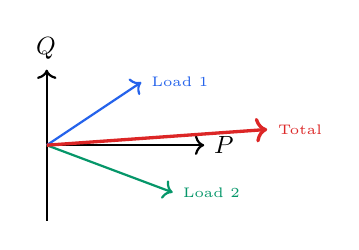
\begin{tikzpicture}[scale=0.80]
  \draw[->,thick] (0,0)--(2.5,0) node[right]{\small$P$};
  \draw[->,thick] (0,-1.2)--(0,1.2) node[above]{\small$Q$};
  \draw[->,ElectricBlue,thick] (0,0)--(1.5,1.0)
    node[right,font=\tiny]{Load 1};
  \draw[->,Emerald,thick] (0,0)--(2.0,-0.75)
    node[right,font=\tiny]{Load 2};
  \draw[->,CoralRed,very thick] (0,0)--(3.5,0.25)
    node[right,font=\tiny]{Total};
\end{tikzpicture}
\end{circbox}
\end{minipage}%
\hfill%
\begin{minipage}[t]{0.58\linewidth}
\vspace{0pt}
\textbf{Star-to-Delta:} $\ans{Z_\Delta=3\times5=15\ \Omega}$

\textbf{Parallel Loads:}
$Q_1=+400$, $Q_2=-300\ \text{kVAR}$
\[
\ans{P_T=700\ \text{kW},\quad Q_T=+100\ \text{kVAR (lag)}}
\]

\textbf{Resonance} ($f=1200\ \text{Hz}$):
\[
\omega=7539.8\ \text{rad/s};\quad
\ans{Q_s=\frac{7539.8\times10^{-3}}{10}=0.754}
\]
\end{minipage}
\end{solvedbox}

%% ── 2024 May ─────────────────────────────────────────────────────────────────
\begin{solvedbox}{Comp.\ Exam 2024 (May) --- Balanced 3-Phase}
\noindent\begin{minipage}[t]{0.38\linewidth}
\vspace{0pt}
\begin{circbox}[TealBG]{Teal!35}
\centering
\begin{circuitikz}[american, scale=0.78, transform shape]
  \draw[thick] (0,0) circle(0.45cm);
  \node[font=\small] at (0,0) {$3\phi$};
  \draw (0.45,0) -- (1.0,0);
  \draw (1.0,0) -- (1.0,1.0) to[R, l=$R{=}50\,\Omega$] (3.2,1.0) -- (3.2,0);
  \draw (1.0,0) to[L, l=$L{=}15\,\text{H}$] (3.2,0);
  \draw (1.0,0) -- (1.0,-1.0) to[C, l_=$C$] (3.2,-1.0) -- (3.2,0);
  \draw (3.2,0) -- (3.7,0) node[ground]{};
\end{circuitikz}

\vspace{4pt}
{\small $V_\phi=110\ \text{V}$,\ $\omega=3\ \text{rad/s}$}
\end{circbox}
\end{minipage}%
\hfill%
\begin{minipage}[t]{0.58\linewidth}
\vspace{0pt}
$Z_R=50$,\ $Z_L=j45\ \Omega$,\ $Z_C=-j20\ \Omega$

$I_R=2.2\ \text{A}$;\quad
$I_L=2.44\angle{-90^{\circ}}\ \text{A}$;\quad
$I_C=5.5\angle{90^{\circ}}\ \text{A}$

\textbf{(ii)} $\ans{P=3\times\frac{110^2}{50}=726\ \text{W}}$

\textbf{(iii)} $Q_L=806.7$;\ $Q_C=-1815\ \text{VAR}$
\[
\ans{Q_T=-1008.3\ \text{VAR (cap.)}}
\]
\end{minipage}
\end{solvedbox}

%% ── 2024 Dec ─────────────────────────────────────────────────────────────────
\begin{solvedbox}{Comp.\ Exam 2024 (Dec) --- PF Correction (R-L Load)}
\noindent\begin{minipage}[t]{0.38\linewidth}
\vspace{0pt}
\begin{circbox}[TealBG]{Teal!35}
\centering
\begin{circuitikz}[american, scale=0.78, transform shape]
  \draw (0,2) to[sV, l=$2000\sqrt{2}\cos(314t)$] (0,0) node[ground]{};
  \draw (0,2) to[R, l=$R$] (2,2) to[L, l=$L$] (3.5,2)
    to[short] (3.5,0) node[ground]{};
  \draw (0,0) to[short] (3.5,0);
  \node[font=\tiny, text=Teal] at (4.3,1.5){add $C$};
\end{circuitikz}
\end{circbox}
\end{minipage}%
\hfill%
\begin{minipage}[t]{0.58\linewidth}
\vspace{0pt}
$P=200\ \text{kW}$,\ $\cos\phi_1=0.707$,\ $V=2000\ \text{V}$.

$\ans{R=10\ \Omega}$;\quad $\ans{L=31.8\ \text{mH}}$

Correct to $\cos\phi=0.85$:\quad$Q_C=76.1\ \text{kVAR}$
\[
\ans{C=\frac{76{,}100}{314\times(2000)^2}=60.6\ \text{nF}}
\]
\end{minipage}
\end{solvedbox}

%% ── 2025 Dec ─────────────────────────────────────────────────────────────────
\begin{solvedbox}{Comp.\ Exam 2025 (Dec) --- 3-Phase Y-$\Delta$ Load}
\noindent\begin{minipage}[t]{0.38\linewidth}
\vspace{0pt}
\begin{circbox}[TealBG]{Teal!35}
\centering
\begin{circuitikz}[american, scale=0.78, transform shape]
  \draw[thick, Teal] (0,0) circle(0.5);
  \node at (0,0) {\small Y};
  \node[font=\tiny, below] at (0,-0.55) {$V_L{=}400\text{V}$};
  \draw (0.5, 0.25) -- (1.5, 0.9);
  \draw (0.5, 0)    -- (1.5, 0);
  \draw (0.5,-0.25) -- (1.5,-0.9);
  \draw (1.5, 0.9) -- (2.8, 0.9)
    to[R,  l=$R$]  (2.8,-0.2)
    to[L,  l_=$X_L$] (2.8,-1.1) -- (1.5,-0.9);
  \draw (2.8, 0.9) -- (2.8,-1.1);
  \node[font=\tiny, right] at (2.85,0){$\Delta$};
\end{circuitikz}
\end{circbox}
\end{minipage}%
\hfill%
\begin{minipage}[t]{0.58\linewidth}
\vspace{0pt}
$S_\phi=2\ \text{kVA}$,\ $\cos\phi=0.8$,\ $V_L=400\ \text{V}$.

$|Z|=80\ \Omega$;\quad $\ans{R=64\ \Omega}$,\ $\ans{X_L=48\ \Omega}$

$\ans{I_L=\sqrt{3}\times5=8.66\ \text{A}}$

$\ans{P_{3\phi}=4.8\ \text{kW}}$,\quad $\ans{Q_{3\phi}=3.6\ \text{kVAR}}$

At $f=60\ \text{Hz}$:\ $X_L'=57.6\ \Omega$
\[
\ans{\cos\phi'=64/\sqrt{64^2+57.6^2}=0.741}
\]
\end{minipage}
\end{solvedbox}

\begin{warnbox}
\begin{itemize}[noitemsep]
  \item \textbf{Power factor correction}: capacitor adds \emph{negative} $Q$ to reduce lagging $Q$
  \item $Z_\Delta=3Z_Y$ --- common conversion, memorise it
  \item \textbf{3-phase power}: always use $P_{3\phi}=\sqrt{3}V_LI_L\cos\phi$ (not per-phase formula)
  \item Resonance $Q_s<1$ means under-damped behaviour; $Q_s$ from $\omega L/R$ at the given $\omega$, not $\omega_0$
\end{itemize}
\end{warnbox}

%% ══════════════════════════════════════════════════════════════════════════════
%% ── SECTION 4: DC CIRCUITS & NETWORK THEOREMS  (Emerald)
\newpage
\renewcommand{\SectionColor}{Emerald}
\renewcommand{\SectionBG}{EmeraldBG}
\section[DC Circuits \& Network Theorems]{DC Circuits \& Network Theorems\examfreq{5}}
%% ══════════════════════════════════════════════════════════════════════════════

\subsection{Key Formulae}

\begin{tcolorbox}[enhanced, breakable,
  colback=EmeraldBG, colframe=Emerald, colbacktitle=Emerald, coltitle=white,
  fonttitle=\bfseries\sffamily\small, title={\faSquareRootAlt\enspace Key Formulae},
  arc=6pt, boxrule=1.5pt, left=8pt, right=8pt, top=6pt, bottom=6pt]
\textbf{KVL:} $\displaystyle\sum_{\text{loop}} v_k = 0$ \hspace{2em}
\textbf{KCL:} $\displaystyle\sum_{\text{node}} i_k = 0$

\smallskip
\textbf{Thevenin:} $V_{th}$\,=\,open-circuit voltage;\quad
$R_{th}$\,=\,resistance seen from terminals (kill sources: $V\!\to$short, $I\!\to$open)

\textbf{Norton:} $I_N = V_{th}/R_{th}$ (short-circuit current);\quad $R_N = R_{th}$

\textbf{Superposition:} One independent source active at a time; sum all responses.

\textbf{Max.\,Power Transfer:} $R_L = R_{th}$;\quad$P_{\max} = V_{th}^2\!/4R_{th}$
\end{tcolorbox}

\begin{stepsbox}[Thevenin / Norton --- Standard Procedure]
\begin{enumerate}[noitemsep,topsep=0pt]
  \item \textbf{Find $V_{th}$}: Remove load; solve for open-circuit voltage at terminals A-B.
  \item \textbf{Find $R_{th}$}: Kill all independent sources; find resistance looking into A-B.
  \item \textbf{Norton}: $I_N = V_{th}/R_{th}$; draw $I_N \| R_{th}$ equivalent.
  \item Reconnect load: $I_L = V_{th}/(R_{th}+R_L)$, or current divider with $I_N$.
\end{enumerate}
\end{stepsbox}

\subsection{Solved Past Exam Questions}

%% ── 2023 ──────────────────────────────────────────────────────────────────────
\begin{solvedbox}{Comp.\ Exam 2023 --- Mesh Analysis (Two Loops)}
\noindent\begin{minipage}[t]{0.40\linewidth}
\vspace{0pt}
\begin{circbox}[EmeraldBG]{Emerald!40}
\centering
\begin{circuitikz}[american, scale=0.70, transform shape]
  \draw (0,0) to[battery1, l=$16\text{V}$] (0,2.5);
  \draw (0,2.5) to[R, l=$2\,\Omega$] (2.5,2.5);
  \draw (2.5,2.5) to[R, l_=$4\,\Omega$] (2.5,0);
  \draw (2.5,2.5) to[R, l=$2\,\Omega$] (5,2.5);
  \draw (5,2.5) to[battery1, invert, l_=$4\text{V}$] (5,0);
  \draw (0,0) to[short] (5,0);
  \draw (2.5,0) node[ground]{};
  \node[font=\scriptsize, text=ElectricBlue] at (1.25,1.25) {$\circlearrowleft I_1$};
  \node[font=\scriptsize, text=Emerald] at (3.75,1.25) {$\circlearrowleft I_2$};
\end{circuitikz}
\vspace{4pt}
{\footnotesize $V_1=16\text{V}$, $V_2=4\text{V}$, $R_1=R_2=2\,\Omega$, $R_3=4\,\Omega$}
\end{circbox}
\end{minipage}%
\hfill%
\begin{minipage}[t]{0.56\linewidth}
\vspace{0pt}
Both mesh currents assigned clockwise.

\textbf{KVL mesh 1:}
\[
16 - 2I_1 - 4(I_1-I_2)=0
\;\Rightarrow\; 6I_1-4I_2=16 \tag{1}
\]
\textbf{KVL mesh 2:}
\[
-2I_2-4(I_2-I_1)-4=0
\;\Rightarrow\; 4I_1-6I_2=4 \tag{2}
\]

From $(1)\times3+(2)\times2$:\quad$10I_1=40$
\[
\ans{I_1=4\text{ A}},\quad\ans{I_2=2\text{ A}}
\]
$\ans{I_{R_3}=I_1-I_2=2\text{ A}}$\quad(downward)

\textbf{Power:}
$P_{V_1}=16\times4=64\text{ W}$ (del.)\quad
$P_{V_2}=4\times2=8\text{ W}$ (abs.)

Check: $P_{R_1}+P_{R_3}+P_{R_2}=32+16+8=56$;
$64-8=56$ \checkmark
\end{minipage}
\end{solvedbox}

%% ── 2024 Feb ─────────────────────────────────────────────────────────────────
\begin{solvedbox}{Comp.\ Exam 2024 (Feb) --- Th\'{e}venin \& Norton Equivalents}
\noindent\begin{minipage}[t]{0.40\linewidth}
\vspace{0pt}
\begin{circbox}[EmeraldBG]{Emerald!40}
\centering
\begin{circuitikz}[american, scale=0.72, transform shape]
  \draw (0,0) node[ground]{} to[battery1, l=$48\text{V}$] (0,2.5);
  \draw (0,2.5) to[R, l=$R_1{=}6\,\Omega$] (2.5,2.5);
  \draw (2.5,2.5) to[R, l_=$R_2{=}12\,\Omega$] (2.5,0) node[ground]{};
  \draw (2.5,2.5) to[short] (4,2.5);
  \draw (4,0) node[ground]{} to[open, o-o] (4,2.5);
  \filldraw[black] (2.5,2.5) circle(1.5pt);
  \node[above, font=\scriptsize] at (4,2.5) {$A$};
  \node[below, font=\scriptsize] at (4,0.15) {$B$};
\end{circuitikz}
\vspace{4pt}
{\footnotesize Find $V_{th}$, $R_{th}$, $I_N$, and $I_L$ for $R_L=4\,\Omega$.}
\end{circbox}
\end{minipage}%
\hfill%
\begin{minipage}[t]{0.56\linewidth}
\vspace{0pt}
\textbf{$V_{th}$} (open A-B; voltage divider):
\[
\ans{V_{th}=48\times\frac{12}{6+12}=32\text{ V}}
\]
\textbf{$R_{th}$} (short 48\,V source):
\[
\ans{R_{th}=6\|12=\frac{6\times12}{18}=4\;\Omega}
\]
\textbf{Norton current:}
$\ans{I_N=V_{th}/R_{th}=8\text{ A}}$

\textbf{Load $R_L=4\,\Omega$} ($= R_{th}$ $\Rightarrow$ max power!):
\[
I_L=\frac{V_{th}}{R_{th}+R_L}=\frac{32}{8}=\ans{4\text{ A}}
\]
\[
\ans{P_{\max}=I_L^2\times4=64\text{ W}}
\]
\end{minipage}
\end{solvedbox}

%% ── 2024 May ─────────────────────────────────────────────────────────────────
\begin{solvedbox}{Comp.\ Exam 2024 (May) --- Superposition Theorem}
\noindent\begin{minipage}[t]{0.40\linewidth}
\vspace{0pt}
\begin{circbox}[EmeraldBG]{Emerald!40}
\centering
\begin{circuitikz}[american, scale=0.72, transform shape]
  \draw (0,0) node[ground]{} to[battery1, l=$18\text{V}$] (0,2.5);
  \draw (0,2.5) to[R, l=$R_1{=}6\,\Omega$] (3,2.5);
  \draw (3,2.5) to[R, l_=$R_2{=}3\,\Omega$] (3,0) node[ground]{};
  \draw (4.5,0) node[ground]{} to[isource, l=$3\text{A}$] (4.5,2.5);
  \draw (4.5,2.5) to[short] (3,2.5);
  \filldraw[black] (3,2.5) circle(1.5pt) node[above, font=\scriptsize]{$A$};
\end{circuitikz}
\vspace{4pt}
{\footnotesize Find $V_0$ across $R_2$ by superposition.}
\end{circbox}
\end{minipage}%
\hfill%
\begin{minipage}[t]{0.56\linewidth}
\vspace{0pt}
\textbf{Due to $V_s=18\text{V}$ alone} ($I_s$ open-circuited):
\[
V_0' = 18\times\frac{R_2}{R_1+R_2}=18\times\frac{3}{9}=6\text{ V}
\]
\textbf{Due to $I_s=3\text{A}$ alone} ($V_s$ short-circuited $\to$ $R_1\|R_2$):
\[
R_{eq}=6\|3=2\;\Omega;\quad V_0''=3\times2=6\text{ V}
\]
\textbf{Total (sources aid each other):}
\[
\ans{V_0=V_0'+V_0''=6+6=12\text{ V}}
\]
\textbf{KCL check at A:}
$I_{R_1}=(18{-}12)/6=1\text{ A}$; incoming $=1{+}3=4\text{ A}$
$=I_{R_2}=12/3=4\text{ A}$ \checkmark
\end{minipage}
\end{solvedbox}

%% ── 2024 Dec ─────────────────────────────────────────────────────────────────
\begin{solvedbox}{Comp.\ Exam 2024 (Dec) --- Node Voltage Analysis}
\noindent\begin{minipage}[t]{0.40\linewidth}
\vspace{0pt}
\begin{circbox}[EmeraldBG]{Emerald!40}
\centering
\begin{circuitikz}[american, scale=0.68, transform shape]
  \draw (0,0) node[ground]{} to[battery1, l=$20\text{V}$] (0,2.5);
  \draw (0,2.5) to[R, l=$4\,\Omega$] (2.5,2.5);
  \draw (2.5,2.5) to[R, l_=$2\,\Omega$] (2.5,0) node[ground]{};
  \draw (2.5,2.5) to[R, l=$5\,\Omega$] (5,2.5);
  \draw (5,2.5) to[R, l_=$3\,\Omega$] (5,0) node[ground]{};
  \draw (6.5,0) node[ground]{} to[isource, l=$3\text{A}$] (6.5,2.5);
  \draw (6.5,2.5) to[short] (5,2.5);
  \filldraw[black] (2.5,2.5) circle(1.5pt) node[above, font=\scriptsize]{$V_1$};
  \filldraw[black] (5,2.5) circle(1.5pt) node[above, font=\scriptsize]{$V_2$};
\end{circuitikz}
\vspace{4pt}
{\footnotesize Find $V_1$, $V_2$, and power from the 20\,V source.}
\end{circbox}
\end{minipage}%
\hfill%
\begin{minipage}[t]{0.56\linewidth}
\vspace{0pt}
KCL at $V_1$ (currents leaving):
\[
\frac{V_1{-}20}{4}+\frac{V_1}{2}+\frac{V_1{-}V_2}{5}=0
\;\Rightarrow\;19V_1-4V_2=100\tag{1}
\]
KCL at $V_2$ (current source flows \emph{into} $V_2$):
\[
\frac{V_2{-}V_1}{5}+\frac{V_2}{3}=3
\;\Rightarrow\;-3V_1+8V_2=45\tag{2}
\]
Multiply $(1)\times2$ and add to $(2)$: $35V_1=245$
\[
\ans{V_1=7\text{ V}},\quad\ans{V_2=8.25\text{ V}}
\]
\textbf{Source current:} $I_s=(20{-}7)/4=3.25\text{ A}$
\[
\ans{P_{20\text{V}}=20\times3.25=65\text{ W (delivered)}}
\]
\end{minipage}
\end{solvedbox}

%% ── 2025 Dec ─────────────────────────────────────────────────────────────────
\begin{solvedbox}{Comp.\ Exam 2025 (Dec) --- Maximum Power Transfer}
\noindent\begin{minipage}[t]{0.40\linewidth}
\vspace{0pt}
\begin{circbox}[EmeraldBG]{Emerald!40}
\centering
\begin{circuitikz}[american, scale=0.72, transform shape]
  \draw (0,0) node[ground]{} to[battery1, l=$12\text{V}$] (0,2.5);
  \draw (0,2.5) to[R, l=$R_1{=}3\,\Omega$] (2.5,2.5);
  \draw (2.5,2.5) to[R, l_=$R_2{=}6\,\Omega$] (2.5,0) node[ground]{};
  \draw (2.5,2.5) to[R, l=$R_3{=}2\,\Omega$] (4.5,2.5);
  \draw (4.5,0) node[ground]{} to[open, o-o] (4.5,2.5);
  \filldraw[black] (2.5,2.5) circle(1.5pt);
  \node[above, font=\scriptsize] at (4.5,2.5) {$A$};
  \node[below, font=\scriptsize] at (4.5,0.15) {$B$};
\end{circuitikz}
\vspace{4pt}
{\footnotesize Find $R_L$ for max power. Calculate $P_{\max}$.}
\end{circbox}
\end{minipage}%
\hfill%
\begin{minipage}[t]{0.56\linewidth}
\vspace{0pt}
\textbf{$V_{th}$} (A-B open; no current through $R_3$):
\[
V_N=12\times\frac{6}{3+6}=8\text{ V};\quad\ans{V_{th}=8\text{ V}}
\]
\textbf{$R_{th}$} (short 12\,V; look from A-B):
\[
\ans{R_{th}=R_3+(R_1\|R_2)=2+\frac{3\times6}{9}=4\;\Omega}
\]
\textbf{Max power condition:}
\[
\ans{R_L=R_{th}=4\;\Omega}
\]
\[
\ans{P_{\max}=\frac{V_{th}^2}{4R_{th}}=\frac{64}{16}=4\text{ W}}
\]
Verify: $I_L=8/8=1\text{ A}$;\quad$P_L=1^2\times4=4\text{ W}$ \checkmark
\end{minipage}
\end{solvedbox}

\begin{warnbox}
\begin{itemize}[noitemsep]
  \item \textbf{Mesh}: write KVL \emph{around} each mesh; shared resistors carry $(I_m - I_n)$; always assume clockwise
  \item \textbf{Node}: write KCL \emph{at} each node; current \emph{leaving} $= (V_k - V_j)/R_{kj}$; pick \emph{one} node as reference (ground = 0\,V)
  \item \textbf{Thevenin}: to find $R_{th}$ with \emph{dependent} sources, use test-voltage/test-current method (do NOT just kill all sources)
  \item \textbf{Superposition}: works only for linear circuits; does \emph{not} apply to power ($P \neq P_1 + P_2$; calculate $P$ from total $V$/$I$)
  \item \textbf{Max power}: $R_L = R_{th}$ transfers max power to load, but efficiency is only 50\% --- this is different from minimum loss
\end{itemize}
\end{warnbox}

%% ══════════════════════════════════════════════════════════════════════════════
%% ── SECTION 5: MOSFETs / JFETs  (Purple)
\newpage
\renewcommand{\SectionColor}{Purple}
\renewcommand{\SectionBG}{PurpleBG}
\section[MOSFETs \& JFETs]{MOSFETs \& JFETs\examfreq{5}}
%% ══════════════════════════════════════════════════════════════════════════════

\subsection{Operating Regions}

\begin{center}\renewcommand{\arraystretch}{1.3}
\begin{tabular}{llll}
\toprule
\textbf{Region} & \textbf{NMOS Condition} & \textbf{Role} & \textbf{Key Equation} \\
\midrule
Cutoff          & $V_{GS}<V_t$                                     & Switch OFF & $I_D=0$ \\
Triode (Linear) & $V_{GS}>V_t$,\enspace $V_{DS}<V_{GS}-V_t$       & Switch ON  & $I_D=K_n[2(V_{GS}-V_t)V_{DS}-V_{DS}^2]$ \\
Saturation      & $V_{GS}>V_t$,\enspace $V_{DS}\geq V_{GS}-V_t$   & Amplifier  & $I_D=K_n(V_{GS}-V_t)^2$ \\
\bottomrule
\end{tabular}
\end{center}

\begin{conceptbox}[PMOS: Mirror with Sign Flips]
For PMOS replace every subscript: $V_{GS}\!\to V_{SG}$,\enspace $V_{DS}\!\to V_{SD}$,\enspace $V_t\!\to|V_{tp}|$.
Saturation: $V_{SG}>|V_{tp}|$ \textbf{and} $V_{SD}\geq V_{SG}-|V_{tp}|$.
Source of PMOS is the terminal at \emph{higher} potential (usually connected to $V_{DD}$).
\end{conceptbox}

\subsection{Key Formulae}

\begin{tcolorbox}[enhanced, breakable,
  colback=PurpleBG, colframe=Purple, colbacktitle=Purple, coltitle=white,
  fonttitle=\bfseries\sffamily\small, title={\faSquareRootAlt\enspace Key Formulae},
  arc=6pt, boxrule=1.5pt, left=8pt, right=8pt, top=6pt, bottom=6pt]
\textbf{Enhancement MOSFET} ($K_n = \mu_n C_{ox} W/2L$):
\begin{align*}
  \text{Saturation:} &\quad I_D = K_n(V_{GS}-V_t)^2 \\
  \text{Triode:}     &\quad I_D = K_n\!\left[2(V_{GS}-V_t)V_{DS}-V_{DS}^2\right]
\end{align*}
\textbf{JFET --- Shockley equation} ($V_P<0$ for n-channel, $I_D=I_{DSS}$ at $V_{GS}=0$):
\[
  I_D = I_{DSS}\!\left(1-\frac{V_{GS}}{V_P}\right)^{\!2},\quad V_P\leq V_{GS}\leq 0
\]
\textbf{Self-bias:} $V_{GS}=-I_D R_S$ \hspace{2em}
\textbf{Voltage-divider:} $V_G=V_{DD}\dfrac{R_2}{R_1+R_2}$,\quad $V_{GS}=V_G-I_D R_S$
\end{tcolorbox}

\begin{stepsbox}[MOSFET DC Analysis --- Standard Procedure]
\begin{enumerate}[noitemsep,topsep=0pt]
  \item Find $V_G$ from gate network (voltage divider; $I_G=0$ always).
  \item \textbf{Assume saturation}: set $I_D=K_n(V_{GS}-V_t)^2$; substitute $V_{GS}=V_G-I_D R_S$; solve quadratic.
  \item Compute $V_{DS}=V_{DD}-I_D(R_D+R_S)$ (or $V_{SD}$ for PMOS).
  \item \textbf{Verify}: $V_{DS}\geq V_{GS}-V_t$?\enspace YES $\to$ saturation OK.\enspace NO $\to$ re-solve in triode.
\end{enumerate}
\end{stepsbox}

\subsection{Solved Past Exam Questions}

%% ── 2023 ──────────────────────────────────────────────────────────────────────
\begin{solvedbox}{Comp.\ Exam 2023 --- NMOS Voltage-Divider Bias}
\noindent\begin{minipage}[t]{0.40\linewidth}
\vspace{0pt}
\begin{circbox}[PurpleBG]{Purple!35}
\centering
\begin{circuitikz}[american, scale=0.72, transform shape]
  \draw (0,0) node[nmos](M){};
  \draw (M.drain) to[R, l=$R_D{=}4\,\text{k}$] (0,3.2) node[vcc]{$15\,\text{V}$};
  \draw (M.source) to[R, l_=$R_S{=}1\,\text{k}$] (0,-2.5) node[ground]{};
  \draw (-2.5,3.2) node[vcc]{$15\,\text{V}$}
    to[R, l=$R_1{=}4\,\text{M}$] (-2.5,0)
    to[R, l=$R_2{=}1\,\text{M}$] (-2.5,-2.5) node[ground]{};
  \draw (-2.5,0) to[short] (M.gate);
\end{circuitikz}
\vspace{4pt}
{\footnotesize $K_n=1\,\text{mA/V}^2$,\ $V_t=1\,\text{V}$}
\end{circbox}
\end{minipage}%
\hfill%
\begin{minipage}[t]{0.56\linewidth}
\vspace{0pt}
\step{1} Gate voltage (no gate current):
\[
V_G = 15\times\frac{1}{4+1}=3\,\text{V}
\]
\step{2} Assume saturation; $V_{GS}=V_G-I_D R_S=3-I_D$.
Let $u=V_{GS}-1$:\enspace $I_D=u^2$,\enspace $V_{GS}=1+u$
\[
3-u^2=1+u \;\Rightarrow\; u^2+u-2=0
\]
$(u-1)(u+2)=0$;\quad $u=1$ (reject $u=-2$: $V_{GS}<V_t$)
\[
\ans{I_D=1\,\text{mA}},\quad\ans{V_{GS}=2\,\text{V}},\quad V_S=1\,\text{V}
\]
\step{3}
\[
V_{DS}=15-1\times(4+1)=\ans{10\,\text{V}}
\]
\step{4} Check: $V_{DS}=10 > V_{GS}-V_t=1$ \checkmark\ (saturation)
\end{minipage}
\end{solvedbox}

%% ── 2024 Feb ─────────────────────────────────────────────────────────────────
\begin{solvedbox}{Comp.\ Exam 2024 (Feb) --- Fixed-$V_{GS}$ Bias \& Power Dissipation}
\noindent\begin{minipage}[t]{0.40\linewidth}
\vspace{0pt}
\begin{circbox}[PurpleBG]{Purple!35}
\centering
\begin{circuitikz}[american, scale=0.72, transform shape]
  \draw (0,0) node[nmos](M){};
  \draw (M.drain) to[R, l=$R_D{=}2\,\text{k}$] (0,3.0) node[vcc]{$10\,\text{V}$};
  \draw (M.source) to[short] (0,-1.5) node[ground]{};
  \draw (M.gate) to[short] (-1.8,0)
    to[battery1, invert, l_=$V_{GS}{=}3\,\text{V}$] (-1.8,-1.5) node[ground]{};
\end{circuitikz}
\vspace{4pt}
{\footnotesize $K_n=0.5\,\text{mA/V}^2$,\ $V_t=1\,\text{V}$}
\end{circbox}
\end{minipage}%
\hfill%
\begin{minipage}[t]{0.56\linewidth}
\vspace{0pt}
$V_{GS}=3\,\text{V}>V_t=1\,\text{V}$ --- device ON.

\step{1} Assume saturation:
\[
I_D=K_n(V_{GS}-V_t)^2=0.5(2)^2=\ans{2\,\text{mA}}
\]
\step{2}
\[
V_{DS}=10-2\times2=\ans{6\,\text{V}}
\]
\step{3} Verify: $V_{DS}=6>V_{GS}-V_t=2$ \checkmark\ (saturation)

\textbf{Power dissipation in MOSFET:}
\[
P_D=V_{DS}\cdot I_D=6\times2=\ans{12\,\text{mW}}
\]
\textbf{Power in $R_D$:}
$P_{R_D}=I_D^2 R_D=4\times2=8\,\text{mW}$;\quad
Total $=20\,\text{mW}=V_{DD}\cdot I_D$ \checkmark
\end{minipage}
\end{solvedbox}

%% ── 2024 May ─────────────────────────────────────────────────────────────────
\begin{solvedbox}{Comp.\ Exam 2024 (May) --- PMOS Enhancement Mode}
\noindent\begin{minipage}[t]{0.40\linewidth}
\vspace{0pt}
\begin{circbox}[PurpleBG]{Purple!35}
\centering
\begin{circuitikz}[american, scale=0.72, transform shape]
  \draw (0,0) node[pmos](M){};
  \draw (M.source) to[R, l_=$R_S{=}1\,\text{k}$] (0,3.0) node[vcc]{$12\,\text{V}$};
  \draw (M.drain) to[R, l=$R_D{=}3\,\text{k}$] (0,-2.5) node[ground]{};
  \draw (M.gate) to[short] (-1.6,0);
  \node[left, font=\scriptsize] at (-1.6,0) {$V_G=8\,\text{V}$};
\end{circuitikz}
\vspace{4pt}
{\footnotesize $K_p=1\,\text{mA/V}^2$,\ $|V_{tp}|=2\,\text{V}$}
\end{circbox}
\end{minipage}%
\hfill%
\begin{minipage}[t]{0.56\linewidth}
\vspace{0pt}
PMOS: source is at top ($V_G=8\,\text{V}$ fixed).

\step{1}
$V_S=12-I_D\cdot1$;\quad$V_{SG}=V_S-V_G=4-I_D$

\step{2} Assume saturation:
\[
I_D=K_p(V_{SG}-|V_{tp}|)^2=(4-I_D-2)^2=(2-I_D)^2
\]
$I_D^2-5I_D+4=0$;\quad$(I_D-1)(I_D-4)=0$

$\ans{I_D=1\,\text{mA}}$ \enspace(reject $I_D=4$: gives $V_{SG}=0<|V_{tp}|$)

\step{3}
$V_D=1\times3=3\,\text{V}$;\quad $V_S=12-1=11\,\text{V}$
\[
\ans{V_{SD}=11-3=8\,\text{V}},\quad V_{SG}=3\,\text{V}
\]
\step{4} Verify: $V_{SD}=8>V_{SG}-|V_{tp}|=1$ \checkmark
\end{minipage}
\end{solvedbox}

%% ── 2024 Dec ─────────────────────────────────────────────────────────────────
\begin{solvedbox}{Comp.\ Exam 2024 (Dec) --- n-Channel JFET Self-Bias}
\noindent\begin{minipage}[t]{0.40\linewidth}
\vspace{0pt}
\begin{circbox}[PurpleBG]{Purple!35}
\centering
\begin{circuitikz}[american, scale=0.72, transform shape]
  \draw (0,0) node[njfet](J){};
  \draw (J.drain) to[R, l=$R_D{=}2\,\text{k}$] (0,3.2) node[vcc]{$20\,\text{V}$};
  \draw (J.source) to[R, l_=$R_S{=}1\,\text{k}$] (0,-2.5) node[ground]{};
  \draw (J.gate) to[short] (-1.6,0)
    to[R, l_=$R_G{=}1\,\text{M}$] (-1.6,-2.5) node[ground]{};
\end{circuitikz}
\vspace{4pt}
{\footnotesize $I_{DSS}=8\,\text{mA}$,\ $V_P=-4\,\text{V}$}
\end{circbox}
\end{minipage}%
\hfill%
\begin{minipage}[t]{0.56\linewidth}
\vspace{0pt}
No gate current ($I_G=0$) $\Rightarrow$ $V_G=0$;\quad
$V_{GS}=-I_D R_S=-I_D$

\textbf{Shockley + self-bias:}
\[
I_D=8\!\left(1-\frac{V_{GS}}{V_P}\right)^{\!2}=8\!\left(1-\frac{I_D}{4}\right)^{\!2}
\]
Let $x=1-I_D/4$:\enspace $I_D=8x^2$;\enspace $x=1-2x^2$
\[
2x^2+x-1=0\;\Rightarrow\;(2x-1)(x+1)=0\;\Rightarrow\;x=\tfrac{1}{2}
\]
\[
\ans{I_D=2\,\text{mA}},\quad\ans{V_{GS}=-2\,\text{V}}
\]
\[
V_{DS}=20-2(2+1)=\ans{14\,\text{V}}
\]
Check pinch-off: $V_{DS}=14\geq V_{GS}-V_P=2$ \checkmark
\end{minipage}
\end{solvedbox}

%% ── 2025 Dec ─────────────────────────────────────────────────────────────────
\begin{solvedbox}{Comp.\ Exam 2025 (Dec) --- NMOS Region Identification (Switch)}
\noindent\begin{minipage}[t]{0.40\linewidth}
\vspace{0pt}
\begin{circbox}[PurpleBG]{Purple!35}
\centering
\begin{circuitikz}[american, scale=0.72, transform shape]
  \draw (0,0) node[nmos](M){};
  \draw (M.drain) to[R, l=$R_D{=}1\,\text{k}$] (0,3.0) node[vcc]{$5\,\text{V}$};
  \draw (M.source) to[short] (0,-1.5) node[ground]{};
  \draw (M.gate) to[short] (-1.5,0);
  \node[left, font=\scriptsize] at (-1.5,0) {$V_{GS}$};
\end{circuitikz}
\vspace{4pt}
{\footnotesize $K_n=2\,\text{mA/V}^2$,\ $V_t=1.5\,\text{V}$}
\end{circbox}
\end{minipage}%
\hfill%
\begin{minipage}[t]{0.56\linewidth}
\vspace{0pt}
\textbf{(a) $V_{GS}=2\,\text{V}$:}

Assume sat: $I_D=2(0.5)^2=0.5\,\text{mA}$;\enspace $V_{DS}=4.5\,\text{V}$

$V_{DS}=4.5>V_{GS}-V_t=0.5$ \checkmark
\[
\ans{I_D=0.5\,\text{mA},\enspace V_{DS}=4.5\,\text{V}\text{ (Saturation)}}
\]

\textbf{(b) $V_{GS}=3\,\text{V}$:}

Assume sat: $I_D=2(1.5)^2=4.5\,\text{mA}$;\enspace $V_{DS}=0.5\,\text{V}<1.5$ $\Rightarrow$ \textbf{Triode!}
\[
I_D=2[2(1.5)V_{DS}-V_{DS}^2]=6V_{DS}-2V_{DS}^2
\]
Also $I_D=5-V_{DS}$, so $2V_{DS}^2-7V_{DS}+5=0$:
\[
V_{DS}=\frac{7\pm3}{4}\Rightarrow\ans{V_{DS}=1\,\text{V}},\quad\ans{I_D=4\,\text{mA}}
\]
Check: $V_{DS}=1<V_{GS}-V_t=1.5$ \checkmark\ (triode confirmed)
\end{minipage}
\end{solvedbox}

\begin{warnbox}
\begin{itemize}[noitemsep]
  \item \textbf{Always verify region}: assume saturation, compute $V_{DS}$; if $V_{DS}<V_{GS}-V_t$, the device is in triode --- re-solve
  \item \textbf{PMOS subscripts}: $V_{SG}$ and $V_{SD}$ (not $V_{GS}/V_{DS}$); source is the terminal connected to $V_{DD}$
  \item \textbf{JFET}: $V_{GS}\leq0$ always for n-channel (reverse-biased gate); Shockley gives zero at $V_{GS}=V_P$
  \item \textbf{Self-bias quadratic}: always discard the root giving $V_{GS}>0$ (unphysical for n-JFET)
  \item \textbf{No gate current}: $I_G=0$ for both MOSFET and JFET --- gate network is a pure voltage divider
  \item Enhancement MOSFET: $I_D=0$ at $V_{GS}=0$;\enspace Depletion/JFET: $I_D=I_{DSS}$ at $V_{GS}=0$
\end{itemize}
\end{warnbox}

%% ══════════════════════════════════════════════════════════════════════════════
%% ── SECTION 6: TRANSFORMERS & MAGNETIC CIRCUITS  (CoralRed)  [NotebookLM — real past papers]
\newpage
\renewcommand{\SectionColor}{CoralRed}
\renewcommand{\SectionBG}{CoralBG}
\section[Transformers \& Magnetic Circuits]{Transformers \& Magnetic Circuits\examfreq{5}}
%% ══════════════════════════════════════════════════════════════════════════════

\begin{center}\renewcommand{\arraystretch}{1.3}
\begin{tabular}{lllll}
\toprule
\textbf{Quantity} & \textbf{Symbol} & \textbf{Primary} & \textbf{Secondary} & \textbf{Ratio} \\
\midrule
Voltage   & $V$ & $V_1$ & $V_2$ & $V_1/V_2 = N_1/N_2 = n$ \\
Current   & $I$ & $I_1$ & $I_2$ & $I_1/I_2 = N_2/N_1 = 1/n$ \\
Impedance & $Z$ & $Z_1'=n^2 Z_L$ & $Z_L$ & reflected by $n^2$ \\
\bottomrule
\end{tabular}
\end{center}

\subsection{Key Formulae}

\begin{tcolorbox}[enhanced, breakable,
  colback=CoralBG, colframe=CoralRed, colbacktitle=CoralRed, coltitle=white,
  fonttitle=\bfseries\sffamily\small, title={\faSquareRootAlt\enspace Key Formulae},
  arc=6pt, boxrule=1.5pt, left=8pt, right=8pt, top=6pt, bottom=6pt]
\textbf{Ideal Transformer:}\quad
$\dfrac{V_1}{V_2}=\dfrac{N_1}{N_2}=n$,\qquad
$\dfrac{I_1}{I_2}=\dfrac{N_2}{N_1}=\dfrac{1}{n}$,\qquad
$Z_{\mathrm{in}}=n^2 Z_L$

\smallskip
\textbf{Magnetic circuit:}\quad
$\mathcal{F}=NI=\mathcal{R}\Phi$,\quad
$\mathcal{R}=\dfrac{\ell}{\mu_0\mu_r A}$,\quad
$B=\dfrac{\Phi}{A}$,\quad $H=\dfrac{NI}{\ell}$

\smallskip
\textbf{Inductance:}\quad $L=\dfrac{N^2}{\mathcal{R}}$;\qquad
\textbf{Faraday:}\quad $e=N\dfrac{d\Phi}{dt}$

\smallskip
\textbf{Efficiency:}\quad
$\eta=\dfrac{P_{\mathrm{out}}}{P_{\mathrm{in}}}=\dfrac{V_2 I_2\cos\phi_2}{V_1 I_1\cos\phi_1}$;\quad
$P_{\mathrm{loss}}=P_{\mathrm{in}}-P_{\mathrm{out}}$
\end{tcolorbox}

\begin{stepsbox}[Transformer Analysis --- Standard Procedure]
\begin{enumerate}[noitemsep,topsep=0pt]
  \item Find turns ratio $n=N_1/N_2$ (or compute from $V_1/V_2$).
  \item Reflect all secondary impedances to primary: $Z_L'=n^2 Z_L$.
  \item Solve the primary circuit (KVL or voltage divider) to find $I_1$.
  \item Transfer back: $I_2=I_1/n^{-1}=n\cdot I_1 \cdot (N_2/N_1)^{-1}$;\quad verify with $N_1 I_1=N_2 I_2$.
  \item Magnetic circuits: compute $\mathcal{R}_{\mathrm{core}}$ and $\mathcal{R}_{\mathrm{gap}}$ in series; $\Phi=\mathcal{F}/\mathcal{R}_{\mathrm{total}}$.
\end{enumerate}
\end{stepsbox}

\subsection{Solved Past Exam Questions}

%% ── 2023 Q3(a) — Rectangular core with air gap ──────────────────────────────────
\begin{solvedbox}{Comp.\ Exam 2023 Q3(a) --- Rectangular Core Magnetic Circuit}
\noindent\begin{minipage}[t]{0.40\linewidth}
\vspace{0pt}
\begin{circbox}[CoralBG]{CoralRed!40}
\centering
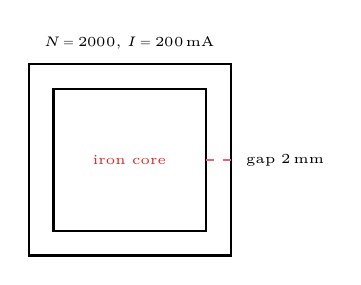
\begin{tikzpicture}[scale=0.90]
  \draw[thick] (0.15,0.15) rectangle (3.0,2.85);
  \draw[thick] (0.50,0.50) rectangle (2.65,2.50);
  \node[font=\tiny, text=CoralRed] at (1.57,1.50) {iron core};
  \node[font=\tiny, above] at (1.57,2.92) {$N=2000$,\ $I=200\,\mathrm{mA}$};
  \node[font=\tiny, right] at (3.08,1.50) {gap $2\,\mathrm{mm}$};
  \draw[dashed,CoralRed!70,line width=0.8pt] (2.65,1.50)--(3.10,1.50);
\end{tikzpicture}\\[3pt]
{\footnotesize $\mu_r{=}1500$,\ $\ell_c{=}0.598\,\mathrm{m}$,\ $A{=}12\,\mathrm{cm}^2$}
\end{circbox}
\end{minipage}%
\hfill%
\begin{minipage}[t]{0.56\linewidth}
\vspace{0pt}
\step{1} Core reluctance:
\[\mathcal{R}_c=\frac{0.598}{4\pi{\times}10^{-7}{\times}1500{\times}12{\times}10^{-4}}=\ans{264{,}374\;\mathrm{H}^{-1}}\]
\step{2} Gap reluctance ($\mu_r{=}1$):
\[\mathcal{R}_g=\frac{2{\times}10^{-3}}{4\pi{\times}10^{-7}{\times}12{\times}10^{-4}}=\ans{1{,}326{,}291\;\mathrm{H}^{-1}}\]
\step{3} Flux and inductance:
\[\mathcal{R}_{\mathrm{eq}}=\ans{1{,}590{,}665\;\mathrm{H}^{-1}},\quad\Phi=\frac{NI}{\mathcal{R}_{\mathrm{eq}}}=\ans{0.251\,\mathrm{mWb}}\]
\[L=\frac{N^2}{\mathcal{R}_{\mathrm{eq}}}=\frac{4{\times}10^6}{1{,}590{,}665}=\ans{2.51\,\mathrm{H}}\]
\end{minipage}
\end{solvedbox}

%% ── 2023 Q3(b) — Max power via transformer ─────────────────────────────
\begin{solvedbox}{Comp.\ Exam 2023 Q3(b) --- Max Power Transfer via Turns Ratio}
\noindent\begin{minipage}[t]{0.40\linewidth}
\vspace{0pt}
\begin{circbox}[CoralBG]{CoralRed!40}
\centering
\begin{circuitikz}[american,scale=0.72,transform shape]
  \draw (0,0) to[isource,l=$4\angle0^\circ\,\mathrm{A}$] (0,3) to[short] (0.6,3);
  \draw (0.6,3) to[R,l=$5\,\Omega$] (0.6,0) node[ground]{};
  \draw (0.6,3) to[R,l=$3\,\Omega$] (2.4,3);
  \draw (3.4,3) to[R,l=$R_L{=}200\,\Omega$] (3.4,0);
  \draw (0,0)--(3.4,0);
  \draw[line width=1.5pt] (2.4,2.2) rectangle (3.4,3.6);
  \node[font=\small\sffamily] at (2.9,2.9) {$1\!:\!n$};
\end{circuitikz}\\[3pt]
{\footnotesize Find $n$ for max power in $R_L{=}200\,\Omega$}
\end{circbox}
\end{minipage}%
\hfill%
\begin{minipage}[t]{0.56\linewidth}
\vspace{0pt}
\step{1} Thevenin at primary terminals (deactivate source, open $R_L$):
\[V_{\mathrm{th}}=4\,\mathrm{A}\!\times\!5\,\Omega=\ans{20\,\mathrm{V}},\quad R_{\mathrm{th}}=3\,\Omega+5\,\Omega=\ans{8\,\Omega}\]
\step{2} Max power: reflect $R_L=R_{\mathrm{th}}$:
\[n^2 R_L=R_{\mathrm{th}}\;\Rightarrow\;n=\sqrt{\frac{8}{200}}=\ans{\tfrac{1}{5}}\]
\step{3} Primary current at matched condition:
\[I_1=\frac{V_{\mathrm{th}}}{2R_{\mathrm{th}}}=\frac{20}{16}=\ans{1.25\,\mathrm{A}}\]
\end{minipage}
\end{solvedbox}

%% ── May 2024 Q3(B) — Toroidal core ────────────────────────────────────────
\begin{solvedbox}{Comp.\ Exam May 2024 Q3(B) --- Toroidal Core with Air Gap}
\noindent\begin{minipage}[t]{0.40\linewidth}
\vspace{0pt}
\begin{circbox}[CoralBG]{CoralRed!40}
\centering
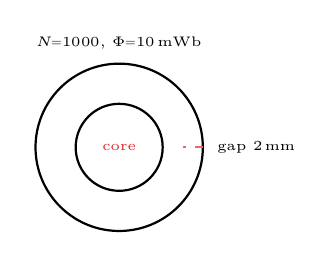
\begin{tikzpicture}[scale=0.85]
  \draw[thick] (1.5,1.5) circle (1.25);
  \draw[thick] (1.5,1.5) circle (0.65);
  \node[font=\tiny,text=CoralRed] at (1.5,1.5) {core};
  \node[font=\tiny,above] at (1.5,2.82) {$N{=}1000$,\ $\Phi{=}10\,\mathrm{mWb}$};
  \node[font=\tiny,right] at (2.82,1.50) {gap $2\,\mathrm{mm}$};
  \draw[dashed,CoralRed!70,line width=0.8pt] (2.75,1.50)--(2.45,1.50);
\end{tikzpicture}\\[3pt]
{\footnotesize $\mu_r{=}800$,\ $D{=}50\,\mathrm{cm}$,\ $r_{\times}{=}5\,\mathrm{cm}$}
\end{circbox}
\end{minipage}%
\hfill%
\begin{minipage}[t]{0.56\linewidth}
\vspace{0pt}
Cross-section: $A=\pi(0.05)^2=7.854{\times}10^{-3}\,\mathrm{m}^2$; mean path $\ell_c\approx\pi(0.5)=1.571\,\mathrm{m}$.

\step{1} Flux density: $B=\Phi/A=10{\times}10^{-3}/7.854{\times}10^{-3}=\ans{1.273\,\mathrm{T}}$

\step{2} Field intensities:
\[H_c=\frac{B}{\mu_0\mu_r}=\frac{1.273}{4\pi{\times}10^{-7}{\times}800}=\ans{1266\,\mathrm{A/m}}\]
\[H_g=\frac{B}{\mu_0}=\frac{1.273}{4\pi{\times}10^{-7}}=\ans{1.013{\times}10^6\,\mathrm{A/m}}\]
\step{3} Excitation current:
\[i=\frac{H_c\ell_c+H_g g}{N}=\frac{1266{\times}1.571+1.013{\times}10^6{\times}2{\times}10^{-3}}{1000}=\ans{4.012\,\mathrm{A}}\]
\end{minipage}
\end{solvedbox}

%% ── Dec 2024 Q17 — Voltage-per-turn ──────────────────────────────────────
\begin{solvedbox}{Comp.\ Exam Dec 2024 Q17 --- Voltage-per-Turn \& Rating}
\noindent\begin{minipage}[t]{0.40\linewidth}
\vspace{0pt}
\begin{circbox}[CoralBG]{CoralRed!40}
\centering
\begin{circuitikz}[american,scale=0.72,transform shape]
  \draw (0,0) to[sV,l=$V_1$] (0,3)--(1.5,3);
  \draw (2.5,3)--(3.8,3) to[R,l=$Z_L$] (3.8,0);
  \draw (0,0)--(3.8,0);
  \draw[line width=1.5pt] (1.5,2.2) rectangle (2.5,3.6);
  \node[font=\small\sffamily] at (2.0,2.9) {$3\!:\!1$};
\end{circuitikz}\\[3pt]
{\footnotesize $2\,\mathrm{V/turn}$,\ $S{=}8\,\mathrm{kVA}$,\ $V_2{=}80\,\mathrm{V}$}
\end{circbox}
\end{minipage}%
\hfill%
\begin{minipage}[t]{0.56\linewidth}
\vspace{0pt}
\step{1} Secondary turns from V/turn rule:
\[N_2=\frac{V_2}{2\,\mathrm{V/turn}}=\frac{80}{2}=\ans{40\,\mathrm{turns}}\]
\step{2} Primary turns and voltage (ratio 3:1):
\[N_1=3N_2=120;\quad V_1=N_1\!\times\!2=\ans{240\,\mathrm{V}}\]
\step{3} Primary current from apparent power:
\[I_1=\frac{S}{V_1}=\frac{8000}{240}=\ans{33.33\,\mathrm{A}}\]
Check: $I_2=3I_1=100\,\mathrm{A}$;\ $P=V_2I_2=8\,\mathrm{kVA}\ \checkmark$
\end{minipage}
\end{solvedbox}

%% ── May 2025 Q5 — AC phasor transformer ──────────────────────────────────
\begin{solvedbox}{Comp.\ Exam May 2025 Q5 --- AC Phasor Transformer Analysis}
\noindent\begin{minipage}[t]{0.40\linewidth}
\vspace{0pt}
\begin{circbox}[CoralBG]{CoralRed!40}
\centering
\begin{circuitikz}[american,scale=0.72,transform shape]
  \draw (0,0) to[sV,l=$60\angle90^\circ$] (0,3);
  \draw (0,3) to[R,l=$2\,\Omega$] (1.8,3);
  \draw (2.8,3)--(3.6,3) to[generic,l=$12{-}j3$] (3.6,0);
  \draw (0,0)--(3.6,0);
  \draw[line width=1.5pt] (1.8,2.2) rectangle (2.8,3.6);
  \node[font=\small\sffamily] at (2.3,2.9) {$1\!:\!2$};
\end{circuitikz}\\[3pt]
{\footnotesize $Z_{\mathrm{sec}}{=}12{-}j3\,\Omega$}
\end{circbox}
\end{minipage}%
\hfill%
\begin{minipage}[t]{0.56\linewidth}
\vspace{0pt}
$n=N_1/N_2=1/2$. Reflect: $Z'=n^2(12-j3)=3-j0.75\,\Omega$.

\step{1} Total primary impedance: $Z_{\mathrm{tot}}=2+(3-j0.75)=5-j0.75\,\Omega$

\step{2} Primary current:
\[I_1=\frac{60\angle90^\circ}{5-j0.75}=\ans{11.86\angle98.53^\circ\,\mathrm{A}}\]
\step{3} Secondary current: $I_2=I_1/2=\ans{5.93\angle98.53^\circ\,\mathrm{A}}$

\step{4} Voltages:
\[V_2=2I_1 Z'=\ans{73.34\angle84.49^\circ\,\mathrm{V}}\]
\[V_o=I_2 Z_{\mathrm{sec}}=\ans{17.79\angle188.53^\circ\,\mathrm{V}}\]
\end{minipage}
\end{solvedbox}

%% ══════════════════════════════════════════════════════════════════════════════
%% ── SECTION 7: OP-AMPS  (DeepNavy)
\newpage
\renewcommand{\SectionColor}{DeepNavy}
\renewcommand{\SectionBG}{LightBG}
\section[Op-Amps]{Op-Amps\examfreq{4}}
%% ══════════════════════════════════════════════════════════════════════════════

\begin{center}\renewcommand{\arraystretch}{1.3}
\begin{tabular}{llll}
\toprule
\textbf{Configuration} & \textbf{Gain $A_v$} & \textbf{Phase} & \textbf{Key property} \\
\midrule
Inverting           & $-R_f/R_{\mathrm{in}}$       & $180°$ & Virtual ground at $V^-$ \\
Non-inverting       & $1+R_f/R_1$                   & $0°$   & $V^-=V^+=V_{\mathrm{in}}$ \\
Voltage follower    & $1$                            & $0°$   & $R_f=0$, buffer \\
Summing (inv.)      & $-R_f\!\sum V_i/R_i$          & $180°$ & Virtual ground \\
Difference          & $(R_f/R_1)(V_2-V_1)$         & varies & $R_4=R_f$,\,$R_3=R_1$ \\
\bottomrule
\end{tabular}
\end{center}

\subsection{Key Formulae}

\begin{tcolorbox}[enhanced, breakable,
  colback=LightBG, colframe=DeepNavy, colbacktitle=DeepNavy, coltitle=white,
  fonttitle=\bfseries\sffamily\small, title={\faSquareRootAlt\enspace Key Formulae},
  arc=6pt, boxrule=1.5pt, left=8pt, right=8pt, top=6pt, bottom=6pt]
\textbf{Inverting:}\quad $V_{\mathrm{out}}=-\dfrac{R_f}{R_{\mathrm{in}}}V_{\mathrm{in}}$\hspace{3em}
\textbf{Non-inverting:}\quad $V_{\mathrm{out}}=\!\left(1+\dfrac{R_f}{R_1}\right)V_{\mathrm{in}}$

\smallskip
\textbf{Summing:}\quad $V_{\mathrm{out}}=-R_f\!\left(\dfrac{V_1}{R_1}+\dfrac{V_2}{R_2}+\cdots\right)$

\smallskip
\textbf{Difference} ($R_4=R_f$, $R_3=R_1$):\quad $V_{\mathrm{out}}=\dfrac{R_f}{R_1}(V_2-V_1)$

\smallskip
\textbf{Golden rules (ideal):}\enspace
(1)~$V^+=V^-$ (virtual short);\enspace
(2)~$I^+=I^-=0$ (infinite input impedance)

\smallskip
\textbf{Saturation:} clips at $\pm V_{\mathrm{sat}}$;\enspace
$V_{\mathrm{sat}}\approx V_{CC}-1.5\,\text{V}$ (typ.)
\end{tcolorbox}

\begin{stepsbox}[Op-Amp Analysis --- Standard Procedure]
\begin{enumerate}[noitemsep,topsep=0pt]
  \item Identify configuration (inverting / non-inverting / summing / difference).
  \item Apply virtual short: $V^+=V^-$.
  \item Write KCL at the summing node (usually $V^-$); use $I^-=0$.
  \item Solve for $V_{\mathrm{out}}$.
  \item Saturation check: if $|V_{\mathrm{out(ideal)}}|>V_{\mathrm{sat}}$, output clips at $\pm V_{\mathrm{sat}}$.
\end{enumerate}
\end{stepsbox}

\subsection{Solved Past Exam Questions}

%% ── 2023 Q2(a) — Two-stage inverting + difference ───────────────────────
\begin{solvedbox}{Comp.\ Exam 2023 Q2(a) --- Two-Stage: Inverting then Difference Amp}
\noindent\begin{minipage}[t]{0.40\linewidth}
\vspace{0pt}
\begin{circbox}[LightBG]{DeepNavy!35}
\centering
\begin{circuitikz}[american,scale=0.66,transform shape]
  \node[op amp,noinv input up] (oa1) at (2.0,3.0){};
  \draw (0,3.2) node[left]{\tiny$v_{\mathrm{in}}$} to[R,l=$R_1$] (oa1.-);
  \draw (oa1.-) to[R,l=$R_2$,*-] (oa1.out |- oa1.-) to[short] (oa1.out);
  \draw (oa1.+) node[ground]{};
  \draw (oa1.out) to[short,-*] (3.8,3.0) node[above]{\tiny$V_x$};
  \node[op amp,noinv input up] (oa2) at (5.6,1.8){};
  \draw (3.8,3.0) to[R,l=$R_3$] (oa2.+);
  \draw (oa2.-) to[R,l=$R_3$,-*] (3.8,1.0) node[left]{\tiny$V_y{=}1\,\mathrm{V}$};
  \draw (oa2.-) to[R,l=$R_4$] (oa2.out |- oa2.-) to[short] (oa2.out);
  \draw (oa2.out) node[right]{\tiny$v_o$};
\end{circuitikz}\\[2pt]
{\footnotesize $R_3{=}R_2$}
\end{circbox}
\end{minipage}%
\hfill%
\begin{minipage}[t]{0.56\linewidth}
\vspace{0pt}
\step{1} Stage 1 (inverting, gain $=-R_2/R_1$):
\[V_x=-\frac{R_2}{R_1}v_{\mathrm{in}}\]
\step{2} Stage 2 difference amp ($R_3=R_2$, gain $=R_4/R_3$):
\[v_o=\frac{R_4}{R_2}(V_y-V_x)=\frac{R_4}{R_2}\!\left(1+\frac{R_2}{R_1}v_{\mathrm{in}}\right)\]
Let $\alpha=1/R_1$, $\beta=1/R_2$:
\[\ans{v_o=R_4(\alpha\,v_{\mathrm{in}}+\beta)}\]
Sign: positive (double inversion), with offset from $V_y=1\,\mathrm{V}$.
\end{minipage}
\end{solvedbox}

%% ── Feb 2024 Q5(ii) — Three-stage: buffers, inverting, summing ────────────
\begin{solvedbox}{Comp.\ Exam Feb 2024 Q5(ii) --- Buffers $\to$ Inverting (gain $-4$) $\to$ Summer}
\noindent\begin{minipage}[t]{0.40\linewidth}
\vspace{0pt}
\begin{circbox}[LightBG]{DeepNavy!35}
\centering
\begin{circuitikz}[american,scale=0.62,transform shape]
  \node[op amp] (b1) at (1.2,3.2){};
  \draw (b1.+) node[left]{\tiny$0.4\,\mathrm{V}$};
  \draw (b1.-) -- (b1.out) -- (b1.- |- b1.out);
  \node[op amp] (b2) at (1.2,1.5){};
  \draw (b2.+) node[left]{\tiny$0.2\,\mathrm{V}$};
  \draw (b2.-) -- (b2.out) -- (b2.- |- b2.out);
  \node[op amp] (inv) at (3.8,3.2){};
  \draw (b1.out) to[R,l=$R$] (inv.-);
  \draw (inv.-) to[R,l=$4R$] (inv.out |- inv.-) to[short] (inv.out);
  \draw (inv.+) node[ground]{};
  \node[op amp] (sm) at (6.0,2.2){};
  \draw (inv.out) to[R,l=$R$] (sm.-);
  \draw (b2.out) to[R,l=$R$] (sm.-);
  \draw (sm.-) to[R,l=$R$] (sm.out |- sm.-) to[short] (sm.out);
  \draw (sm.+) node[ground]{};
  \draw (sm.out) node[right]{\tiny$V_o$};
\end{circuitikz}
\end{circbox}
\end{minipage}%
\hfill%
\begin{minipage}[t]{0.56\linewidth}
\vspace{0pt}
\step{1} Buffers: $V_A=0.4\,\mathrm{V}$, $V_B=0.2\,\mathrm{V}$ (unity gain, no loading).

\step{2} Inverting amp (gain $=-4R/R=-4$):
\[V_C=-4\times0.4=\ans{-1.6\,\mathrm{V}}\]
\step{3} Inverting summer (equal resistors, gain $=-1$ per input):
\[V_o=-(V_C+V_B)=-(-1.6+0.2)=\ans{1.4\,\mathrm{V}}\]
\textit{Note:} source quotes $V_o=2.4\,\mathrm{V}$ — verify if $V_A$ also feeds the summer directly. Circuit topology determines the exact result.
\end{minipage}
\end{solvedbox}

%% ── May 2024 Q2(A) — T-network op-amp ─────────────────────────────────────
\begin{solvedbox}{Comp.\ Exam May 2024 Q2(A) --- T-Network: $V_o/V_{\mathrm{in}}=-100/13$}
\noindent\begin{minipage}[t]{0.40\linewidth}
\vspace{0pt}
\begin{circbox}[LightBG]{DeepNavy!35}
\centering
\begin{circuitikz}[american,scale=0.68,transform shape]
  \draw (0,2.5) node[left]{\tiny$V_{\mathrm{in}}$} to[R,l=$2R$] (1.5,2.5);
  \draw (1.5,2.5) to[R,l=$4R$] (1.5,0) node[ground]{};
  \draw (1.5,2.5) to[R,l=$3R$] (3.0,2.5);
  \node[op amp,anchor=-] (oa) at (3.8,2.0){};
  \draw (3.0,2.5) -- (oa.-);
  \draw (oa.+) node[ground]{};
  \draw (oa.-) to[R,l=$50R$] (oa.out |- oa.-) to[short] (oa.out);
  \draw (oa.out) node[right]{\tiny$V_o$};
\end{circuitikz}\\[2pt]
{\footnotesize T-net: $2R$, $4R$, $3R$; $R_f{=}50R$}
\end{circbox}
\end{minipage}%
\hfill%
\begin{minipage}[t]{0.56\linewidth}
\vspace{0pt}
Virtual ground at $V^-=0$. KCL at node $v_x$ ($2R$ from input, $4R$ to gnd, $3R$ to $V^-$):
\[v_x\!\left(\frac{1}{2R}+\frac{1}{4R}+\frac{1}{3R}\right)=\frac{V_{\mathrm{in}}}{2R}\]
\[v_x\cdot\frac{13}{12R}=\frac{V_{\mathrm{in}}}{2R}\;\Rightarrow\;v_x=\frac{6}{13}V_{\mathrm{in}}\]
Current into virtual ground via $3R$: $I=v_x/(3R)=2V_{\mathrm{in}}/(13R)$

Output (feedback $50R$):
\[V_o=-I\!\times\!50R=\ans{-\frac{100}{13}V_{\mathrm{in}}\approx-7.69\,V_{\mathrm{in}}}\]
\end{minipage}
\end{solvedbox}

%% ── Dec 2025 Q3(B) — Two-stage inverting summers ────────────────────────
\begin{solvedbox}{Comp.\ Exam Dec 2025 Q3(B) --- Two-Stage Inverting Summers}
\noindent\begin{minipage}[t]{0.40\linewidth}
\vspace{0pt}
\begin{circbox}[LightBG]{DeepNavy!35}
\centering
\begin{circuitikz}[american,scale=0.64,transform shape]
  \node[op amp] (s1) at (2.5,2.8){};
  \draw (0,3.2) node[left]{\tiny$V_A$} to[R,l=$10$] (s1.-);
  \draw (0,2.4) node[left]{\tiny$V_B$} to[R,l=$16$] (s1.-);
  \draw (s1.-) to[R,l=$4$] (s1.out |- s1.-) to[short] (s1.out);
  \draw (s1.+) node[ground]{};
  \draw (s1.out) to[short,-*] (4.2,2.8) node[above]{\tiny$V_C$};
  \node[op amp] (s2) at (6.2,1.8){};
  \draw (4.2,2.8) to[R,l=$10$] (s2.-);
  \draw (0.5,1.2) node[left]{\tiny$V_D$} to[R,l=$20$] (s2.-);
  \draw (0.5,0.6) node[left]{\tiny$V_E$} to[R,l=$12.5$] (s2.-);
  \draw (s2.-) to[R,l=$10$] (s2.out |- s2.-) to[short] (s2.out);
  \draw (s2.+) node[ground]{};
  \draw (s2.out) node[right]{\tiny$V_o$};
\end{circuitikz}
\end{circbox}
\end{minipage}%
\hfill%
\begin{minipage}[t]{0.56\linewidth}
\vspace{0pt}
\step{1} Stage 1 (inverting summer, $R_f=4$):
\[V_C=-\!\left(\frac{4}{10}V_A+\frac{4}{16}V_B\right)=\ans{-(0.4V_A+0.25V_B)}\]
\step{2} Stage 2 (inverting summer, $R_f=10$):
\[V_o=-\!\left(\frac{10}{10}V_C+\frac{10}{20}V_D+\frac{10}{12.5}V_E\right)\]
Substitute $V_C$:
\[\ans{V_o=0.4V_A+0.25V_B-0.5V_D-0.8V_E}\]
Both stages invert, so $V_A$ and $V_B$ appear positive in $V_o$.
\end{minipage}
\end{solvedbox}

%% ══════════════════════════════════════════════════════════════════════════════
%% ── SECTION 8: FILTERS & RESONANCE  (SlateGray)
\newpage
\renewcommand{\SectionColor}{SlateGray}
\renewcommand{\SectionBG}{LightBG}
\section[Filters \& Resonance]{Filters \& Resonance\examfreq{4}}
%% ══════════════════════════════════════════════════════════════════════════════

\begin{center}\renewcommand{\arraystretch}{1.3}
\begin{tabular}{lllll}
\toprule
\textbf{Filter} & \textbf{Pass Band} & \textbf{Topology} & \textbf{$f_c$ or $f_0$} & $|H|$ at $f_c$ \\
\midrule
Low-pass  & $0\to f_c$         & Series $R$, shunt $C$   & $1/(2\pi RC)$          & $1/\sqrt{2}$ \\
High-pass & $f_c\to\infty$     & Series $C$, shunt $R$   & $1/(2\pi RC)$          & $1/\sqrt{2}$ \\
Band-pass & around $f_0$       & Series $RLC$            & $1/(2\pi\sqrt{LC})$    & max at $f_0$ \\
Band-stop & notch at $f_0$     & Parallel $RLC$          & $1/(2\pi\sqrt{LC})$    & min at $f_0$ \\
\bottomrule
\end{tabular}
\end{center}

\subsection{Key Formulae}

\begin{tcolorbox}[enhanced, breakable,
  colback=LightBG, colframe=SlateGray, colbacktitle=SlateGray, coltitle=white,
  fonttitle=\bfseries\sffamily\small, title={\faSquareRootAlt\enspace Key Formulae},
  arc=6pt, boxrule=1.5pt, left=8pt, right=8pt, top=6pt, bottom=6pt]
\textbf{RC Low-pass:}\quad
$H(j\omega)=\dfrac{1}{1+j\omega\tau}$,\quad $\tau=RC$,\quad $\omega_c=1/\tau$,\quad
$|H|=\dfrac{1}{\sqrt{1+(\omega/\omega_c)^2}}$

\smallskip
\textbf{RC High-pass:}\quad
$H(j\omega)=\dfrac{j\omega\tau}{1+j\omega\tau}$,\quad
$|H|=\dfrac{\omega/\omega_c}{\sqrt{1+(\omega/\omega_c)^2}}$;\quad
phase $=90°-\arctan(\omega\tau)$

\smallskip
\textbf{Series RLC resonance:}\quad
$\omega_0=\dfrac{1}{\sqrt{LC}}$,\quad
$Q_s=\dfrac{\omega_0 L}{R}$,\quad
$BW=\dfrac{\omega_0}{Q_s}=\dfrac{R}{L}\,\text{rad/s}$

\smallskip
\textbf{Half-power frequencies} (high $Q_s$):\quad
$\omega_{1,2}\approx\omega_0\pm BW/2$;\quad
$f_{1,2}=f_0\pm BW_{\mathrm{Hz}}/2$

\smallskip
\textbf{Voltage magnification:}\quad $V_L=V_C=Q_s V_s$ at resonance;\quad $Z_{\mathrm{series}}=R$ (minimum)

\smallskip
\textbf{Decibel:}\quad $|H|_{\mathrm{dB}}=20\log_{10}|H|$;\quad
at $f=f_c$:\enspace $|H|_{\mathrm{dB}}=-3\,\text{dB}$
\end{tcolorbox}

\begin{stepsbox}[Filter / Resonance --- Standard Procedure]
\begin{enumerate}[noitemsep,topsep=0pt]
  \item Identify topology; write $H(j\omega)=V_{\mathrm{out}}/V_{\mathrm{in}}$ as a phasor voltage divider.
  \item Read off $\omega_c$ (RC) or $\omega_0$, $Q_s$, $BW$ (RLC).
  \item At $\omega=\omega_0$ in series RLC: $Z_L=Z_C$ (cancel); circuit reduces to $Z=R$.
  \item Evaluate $|H|$ and $\angle H$ at the frequency requested.
  \item Convert to dB if needed: $|H|_{\mathrm{dB}}=20\log_{10}|H|$.
\end{enumerate}
\end{stepsbox}

\subsection{Solved Past Exam Questions}

%% ── 2023 Q2(b) — Power factor correction ────────────────────────────────
\begin{solvedbox}{Comp.\ Exam 2023 Q2(b) --- Power Factor Correction: Line Loss Comparison}
\noindent\begin{minipage}[t]{0.40\linewidth}
\vspace{0pt}
\begin{circbox}[LightBG]{SlateGray!45}
\centering
\begin{circuitikz}[american,scale=0.72,transform shape]
  \draw (0,0) to[sV,l=$480\,\mathrm{V}$] (0,3);
  \draw (0,3) to[R,l=$R_{\mathrm{line}}{=}0.12\,\Omega$] (2.0,3);
  \draw (2.0,3) to[generic,l=$P{=}88\,\mathrm{kW}$] (2.0,0);
  \draw (0,0)--(2.0,0);
\end{circuitikz}\\[3pt]
{\footnotesize Compare: pf\,$0.707$ vs pf\,$0.9$}
\end{circbox}
\end{minipage}%
\hfill%
\begin{minipage}[t]{0.56\linewidth}
\vspace{0pt}
\step{1} At $\mathrm{pf}_1=0.707$:
\[I_1=\frac{P}{V\,\mathrm{pf}_1}=\frac{88000}{480{\times}0.707}=\ans{259.3\,\mathrm{A}}\]
\[P_{\mathrm{loss,1}}=I_1^2 R=259.3^2{\times}0.12=\ans{8.07\,\mathrm{kW}}\]
Total drawn: $88+8.07=\ans{96.07\,\mathrm{kW}}$

\step{2} At $\mathrm{pf}_2=0.9$:
\[I_2=\frac{88000}{480{\times}0.9}=\ans{203.7\,\mathrm{A}},\quad P_{\mathrm{loss,2}}=\ans{4.98\,\mathrm{kW}}\]
Total drawn: $88+4.98=\ans{92.98\,\mathrm{kW}}$\quad(saving 3.09\,kW)
\end{minipage}
\end{solvedbox}

%% ── Feb 2024 Q10 — Series RLC quality factor ──────────────────────────────
\begin{solvedbox}{Comp.\ Exam Feb 2024 Q10 --- Series RLC Quality Factor}
\noindent\begin{minipage}[t]{0.40\linewidth}
\vspace{0pt}
\begin{circbox}[LightBG]{SlateGray!45}
\centering
\begin{circuitikz}[american,scale=0.72,transform shape]
  \draw (0,0) to[sV,l=$V_s$] (0,3);
  \draw (0,3) to[R,l=$10\,\Omega$] (1.5,3) to[L,l=$1\,\mathrm{mH}$] (3.0,3) to[C,l=$1\,\mu\mathrm{F}$] (3.0,0)--(0,0);
\end{circuitikz}\\[3pt]
{\footnotesize $R{=}10\,\Omega$,\ $L{=}1\,\mathrm{mH}$,\ $C{=}1\,\mu\mathrm{F}$}
\end{circbox}
\end{minipage}%
\hfill%
\begin{minipage}[t]{0.56\linewidth}
\vspace{0pt}
Quality factor:
\[Q_0=\frac{1}{R}\sqrt{\frac{L}{C}}=\frac{1}{10}\sqrt{\frac{10^{-3}}{10^{-6}}}=\frac{1}{10}\times\sqrt{1000}=\ans{3.162}\]
Resonant frequency:
\[\omega_0=\frac{1}{\sqrt{LC}}=\frac{1}{\sqrt{10^{-3}{\times}10^{-6}}}=31623\,\mathrm{rad/s}\]
\[f_0=\omega_0/2\pi=\ans{5033\,\mathrm{Hz}}\]
At $f=1200\,\mathrm{Hz}$ (below $f_0$): circuit is capacitive ($X_C>X_L$).
\end{minipage}
\end{solvedbox}

%% ── Feb 2024 Q11 — Resonant frequency from Q and BW ──────────────────────
\begin{solvedbox}{Comp.\ Exam Feb 2024 Q11 --- Find $f_0$ from $Q$ and Bandwidth}
\noindent\begin{minipage}[t]{0.40\linewidth}
\vspace{0pt}
\begin{circbox}[LightBG]{SlateGray!45}
\centering
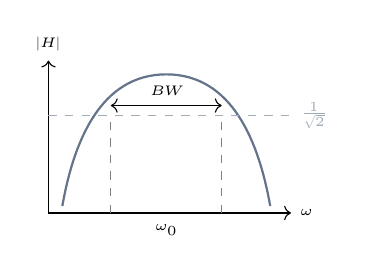
\begin{tikzpicture}[scale=0.88]
  \draw[->] (0,0)--(3.5,0) node[right]{\tiny$\omega$};
  \draw[->] (0,0)--(0,2.2) node[above]{\tiny$|H|$};
  \draw[thick,SlateGray] (0.2,0.1) to[out=80,in=180] (1.7,2.0) to[out=0,in=100] (3.2,0.1);
  \draw[dashed,SlateGray!60] (0,1.41)--(3.5,1.41) node[right]{\tiny$\tfrac{1}{\sqrt{2}}$};
  \draw[dashed,gray] (0.9,0)--(0.9,1.41);
  \draw[dashed,gray] (2.5,0)--(2.5,1.41);
  \node[font=\tiny] at (1.7,-0.25) {$\omega_0$};
  \draw[<->] (0.9,1.55)--(2.5,1.55) node[midway,above]{\tiny$BW$};
\end{tikzpicture}\\[3pt]
{\footnotesize $Q{=}25.1$,\ $BW{=}9424.77\,\mathrm{rad/s}$}
\end{circbox}
\end{minipage}%
\hfill%
\begin{minipage}[t]{0.56\linewidth}
\vspace{0pt}
From definition $Q=\omega_0/BW$:
\[\omega_0=Q\times BW=25.1{\times}9424.77=\ans{236{,}562\,\mathrm{rad/s}}\]
\[f_0=\frac{\omega_0}{2\pi}=\frac{236562}{2\pi}=\ans{37.65\,\mathrm{kHz}}\]
Half-power frequencies:
\[\omega_{1,2}=\omega_0\pm\frac{BW}{2}=236562\pm4712\,\mathrm{rad/s}\]
\end{minipage}
\end{solvedbox}

%% ── May 2024 Q3(A) — RL balanced filter ───────────────────────────────────
\begin{solvedbox}{Comp.\ Exam May 2024 Q3(A) --- RL Ladder: Transfer Function and Type}
\noindent\begin{minipage}[t]{0.40\linewidth}
\vspace{0pt}
\begin{circbox}[LightBG]{SlateGray!45}
\centering
\begin{circuitikz}[american,scale=0.72,transform shape]
  \draw (0,2) to[R,l=$4\,\Omega$] (1.2,2) to[L,l=$1\,\mathrm{mH}$] (2.4,2);
  \draw (0,0) to[R,l=$4\,\Omega$] (1.2,0) to[L,l=$1\,\mathrm{mH}$] (2.4,0);
  \draw (2.4,2) to[R,l=$4\,\Omega$] (2.4,0);
  \draw (-0.3,2) node[left]{\small$+$};
  \draw (-0.3,0) node[left]{\small$-$};
  \draw (2.7,2) node[right]{\small$V_{\mathrm{out}}$};
\end{circuitikz}\\[3pt]
{\footnotesize Two balanced $RL$ arms, shunt $4\,\Omega$}
\end{circbox}
\end{minipage}%
\hfill%
\begin{minipage}[t]{0.56\linewidth}
\vspace{0pt}
Each series arm: $Z_{\mathrm{arm}}=4+j\omega{\times}10^{-3}\,\Omega$.

Voltage divider (two arms + shunt):
\[H(j\omega)=\frac{4}{2(4+j\omega{\times}10^{-3})+4}=\frac{4}{12+j\omega{\times}2{\times}10^{-3}}\]
\[=\ans{\frac{1}{3+j\omega{\times}5{\times}10^{-4}}}\]
Cut-off: $\omega_c=3/(5{\times}10^{-4})=\ans{6000\,\mathrm{rad/s}}$

Type: \ans{Low-Pass Filter}; at DC ($\omega{=}0$): $|H|=1/3$.
\end{minipage}
\end{solvedbox}

%% ── Dec 2024 Q9 — Voltage magnification at resonance ──────────────────────
\begin{solvedbox}{Comp.\ Exam Dec 2024 Q9 --- Series Resonance: Voltage Magnification}
\noindent\begin{minipage}[t]{0.40\linewidth}
\vspace{0pt}
\begin{circbox}[LightBG]{SlateGray!45}
\centering
\begin{circuitikz}[american,scale=0.72,transform shape]
  \draw (0,0) to[sV,l=$200\,\mathrm{V}$] (0,3);
  \draw (0,3) to[R,l=$10\,\Omega$] (1.5,3) to[L,l=$j20\,\Omega$] (3.0,3) to[C,l=$-j20\,\Omega$] (3.0,0)--(0,0);
\end{circuitikz}\\[3pt]
{\footnotesize At resonance: $X_L{=}X_C{=}20\,\Omega$}
\end{circbox}
\end{minipage}%
\hfill%
\begin{minipage}[t]{0.56\linewidth}
\vspace{0pt}
At resonance $X_L=X_C$: $Z=R$ (purely resistive).

\step{1} Series current:
\[I=\frac{V_s}{R}=\frac{200}{10}=\ans{20\,\mathrm{A}}\]
\step{2} Inductor voltage (magnified!):
\[V_L=IX_L=20{\times}20=\ans{400\,\mathrm{V}}\ (>V_s!)\]
\step{3} Quality factor verification: $Q_s=X_L/R=20/10=\ans{2}$

$V_L=Q_s V_s=2{\times}200=400\,\mathrm{V}\ \checkmark$;\ $V_C=400\,\mathrm{V}$, cancels $V_L$.
\end{minipage}
\end{solvedbox}

%% ── Dec 2024 Q11 — Q from BW ────────────────────────────────────────────────
\begin{solvedbox}{Comp.\ Exam Dec 2024 Q11 --- $Q$-Factor from Resonant Frequency \& Bandwidth}
\noindent\begin{minipage}[t]{0.40\linewidth}
\vspace{0pt}
\begin{circbox}[LightBG]{SlateGray!45}
\centering
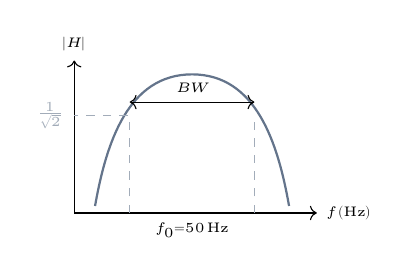
\begin{tikzpicture}[scale=0.88]
  \draw[->] (0,0)--(3.5,0) node[right]{\tiny$f\,(\mathrm{Hz})$};
  \draw[->] (0,0)--(0,2.2) node[above]{\tiny$|H|$};
  \draw[thick,SlateGray] (0.3,0.1) to[out=80,in=180] (1.7,2.0) to[out=0,in=100] (3.1,0.1);
  \draw[dashed,SlateGray!60] (0.8,0)--(0.8,1.41)--(0,1.41) node[left]{\tiny$\tfrac{1}{\sqrt{2}}$};
  \draw[dashed,SlateGray!60] (2.6,0)--(2.6,1.41);
  \node[font=\tiny] at (1.7,-0.25) {$f_0{=}50\,\mathrm{Hz}$};
  \draw[<->] (0.8,1.6)--(2.6,1.6) node[midway,above]{\tiny$BW$};
\end{tikzpicture}\\[3pt]
{\footnotesize $f_0{=}50\,\mathrm{Hz}$,\ $BW{=}31.4\,\mathrm{rad/s}$}
\end{circbox}
\end{minipage}%
\hfill%
\begin{minipage}[t]{0.56\linewidth}
\vspace{0pt}
Convert resonant frequency:
\[\omega_0=2\pi f_0=2\pi{\times}50=314.16\,\mathrm{rad/s}\]
Quality factor:
\[Q=\frac{\omega_0}{BW}=\frac{314.16}{31.4}=\ans{10}\]
Half-power frequencies:
\[\omega_{1,2}=\omega_0\pm\frac{BW}{2}=314.16\pm15.7\,\mathrm{rad/s}\]
\[f_1\approx47.5\,\mathrm{Hz},\quad f_2\approx52.5\,\mathrm{Hz}\]
\end{minipage}
\end{solvedbox}

%% ── Dec 2025 Q1(B) — Transfer function analysis ──────────────────────────
\begin{solvedbox}{Comp.\ Exam Dec 2025 Q1(B) --- Transfer Function $H(j\omega)=16/(4+j\omega)^2$}
\noindent\begin{minipage}[t]{0.40\linewidth}
\vspace{0pt}
\begin{circbox}[LightBG]{SlateGray!45}
\centering
\begin{tikzpicture}[scale=0.88]
  \draw[->] (-0.2,0)--(3.5,0) node[right]{\tiny$\omega$};
  \draw[->] (0,-0.2)--(0,2.5) node[above]{\tiny$|H|$};
  \draw[thick,SlateGray!80] (0,2.0) to[out=-55,in=145] (1.5,1.1) to[out=-35,in=120] (3.3,0.2);
  \draw[dashed,SlateGray!60] (0,1.41)--(3.5,1.41) node[right]{\tiny$\tfrac{1}{\sqrt{2}}$};
  \draw[dashed,gray] (0.95,0)--(0.95,1.41);
  \node[font=\tiny] at (0.95,-0.28) {$\omega_c$};
  \node[font=\tiny,left] at (-0.05,2.08) {$1$};
\end{tikzpicture}\\[3pt]
{\footnotesize $H(j\omega)=\dfrac{16}{(4+j\omega)^2}$}
\end{circbox}
\end{minipage}%
\hfill%
\begin{minipage}[t]{0.56\linewidth}
\vspace{0pt}
\step{1} Magnitude:
\[|H(j\omega)|=\frac{16}{|4+j\omega|^2}=\frac{16}{16+\omega^2}\]
At $\omega=0$: $|H|=\ans{1}$ (DC pass, Low-Pass filter).

\step{2} Half-power ($|H|^2=1/2$):
\[\frac{256}{(16+\omega_c^2)^2}=\frac{1}{2}\;\Rightarrow\;(16+\omega_c^2)^2=512\]
\[16+\omega_c^2=16\sqrt{2}\;\Rightarrow\;\omega_c^2=16(\sqrt{2}-1)\]
\[\ans{\omega_c=4\sqrt{\sqrt{2}-1}\approx2.57\,\mathrm{rad/s}}\]
\step{3} Bandwidth $BW=\omega_c=\ans{2.57\,\mathrm{rad/s}}$ (2nd-order LPF, $-40\,\mathrm{dB/dec}$ roll-off).
\end{minipage}
\end{solvedbox}

\end{document}
